\section{產品與服務內容}

\subsection{服務內容}

普羅程式將提供程式教學工具的開發與服務,以及產品 ProgLearn 程式教學系統。

\subsection{產品}

ProgLearn程式教學系統(以下簡稱為本系統),以程式教師為中心設計,強調師生間的即時互動,提供低延遲直播、課程與作業管理,以及具有即時反饋功能的數位儀表板、講義視覺化編輯、智慧引導和自動批改等多功能(圖\ref{fig:Classroom})。

\begin{figure}[H]
  \begin{subfigure}{0.5\linewidth}
    \centering
    %   \href{https://raw.githubusercontent.com/programingtw/proglearn-plan/main/img/student.png}{ 
    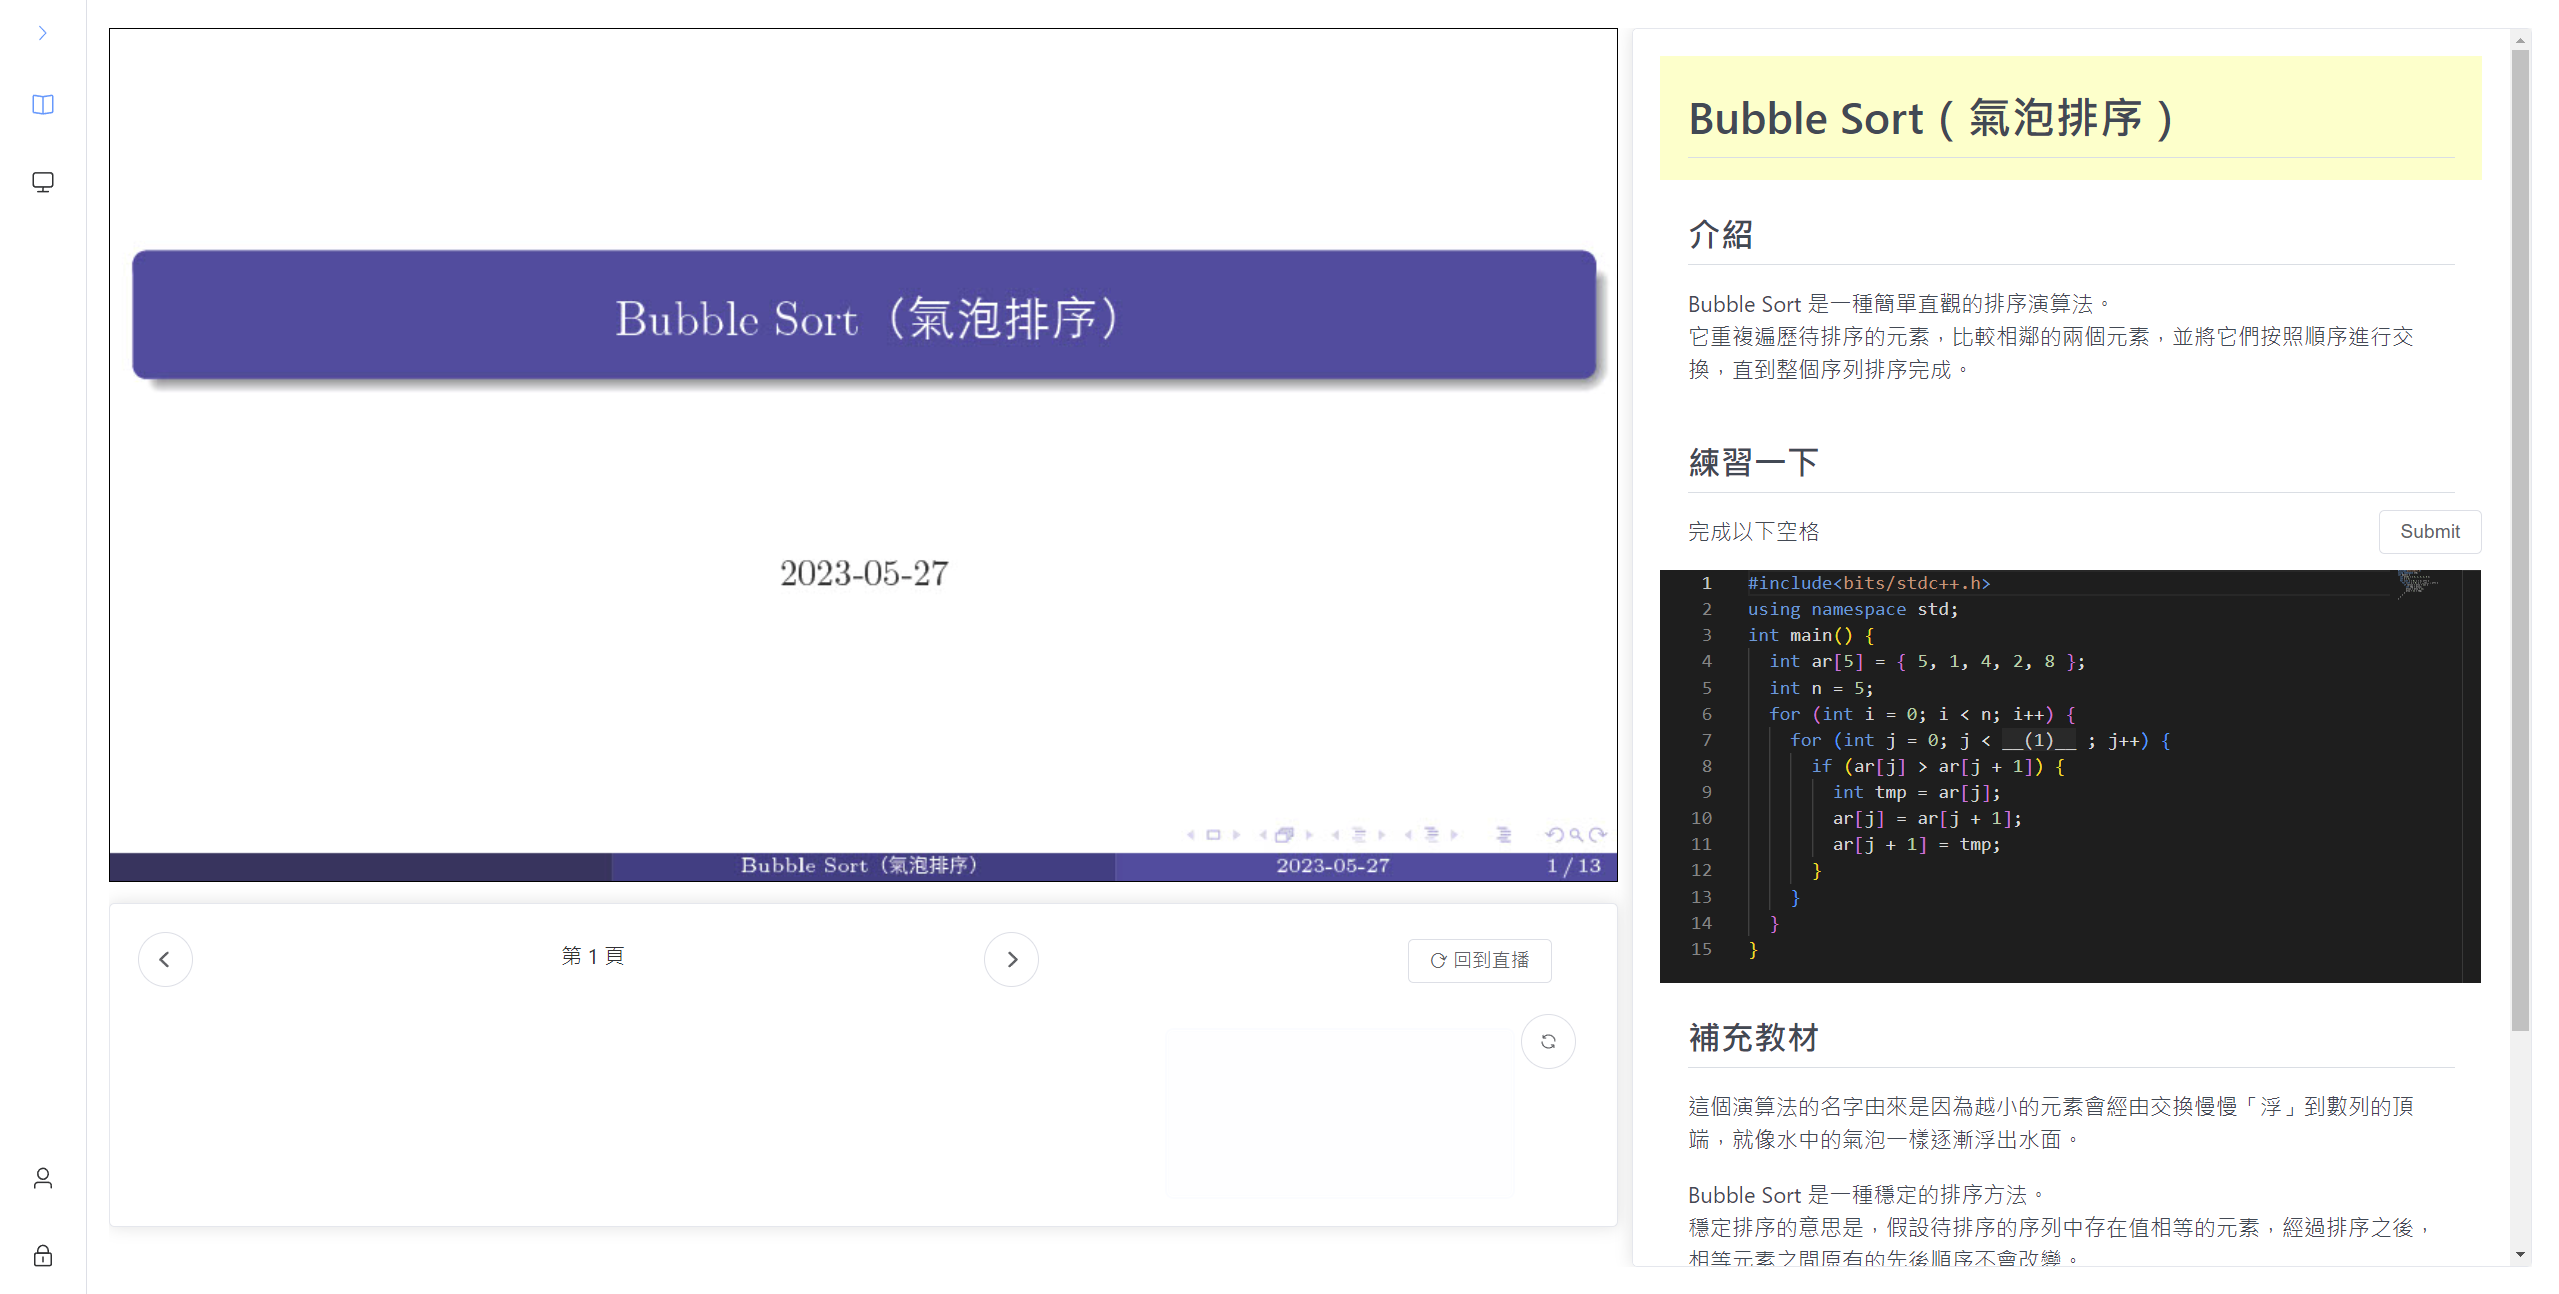
\includegraphics[width=1\textwidth]{images/student.png}
    %   }
    \caption{學生課堂頁面}
  \end{subfigure}
  \begin{subfigure}{0.5\linewidth}
    \centering
        % \href{https://raw.githubusercontent.com/programingtw/proglearn-plan/main/img/teacher.png}{ 
    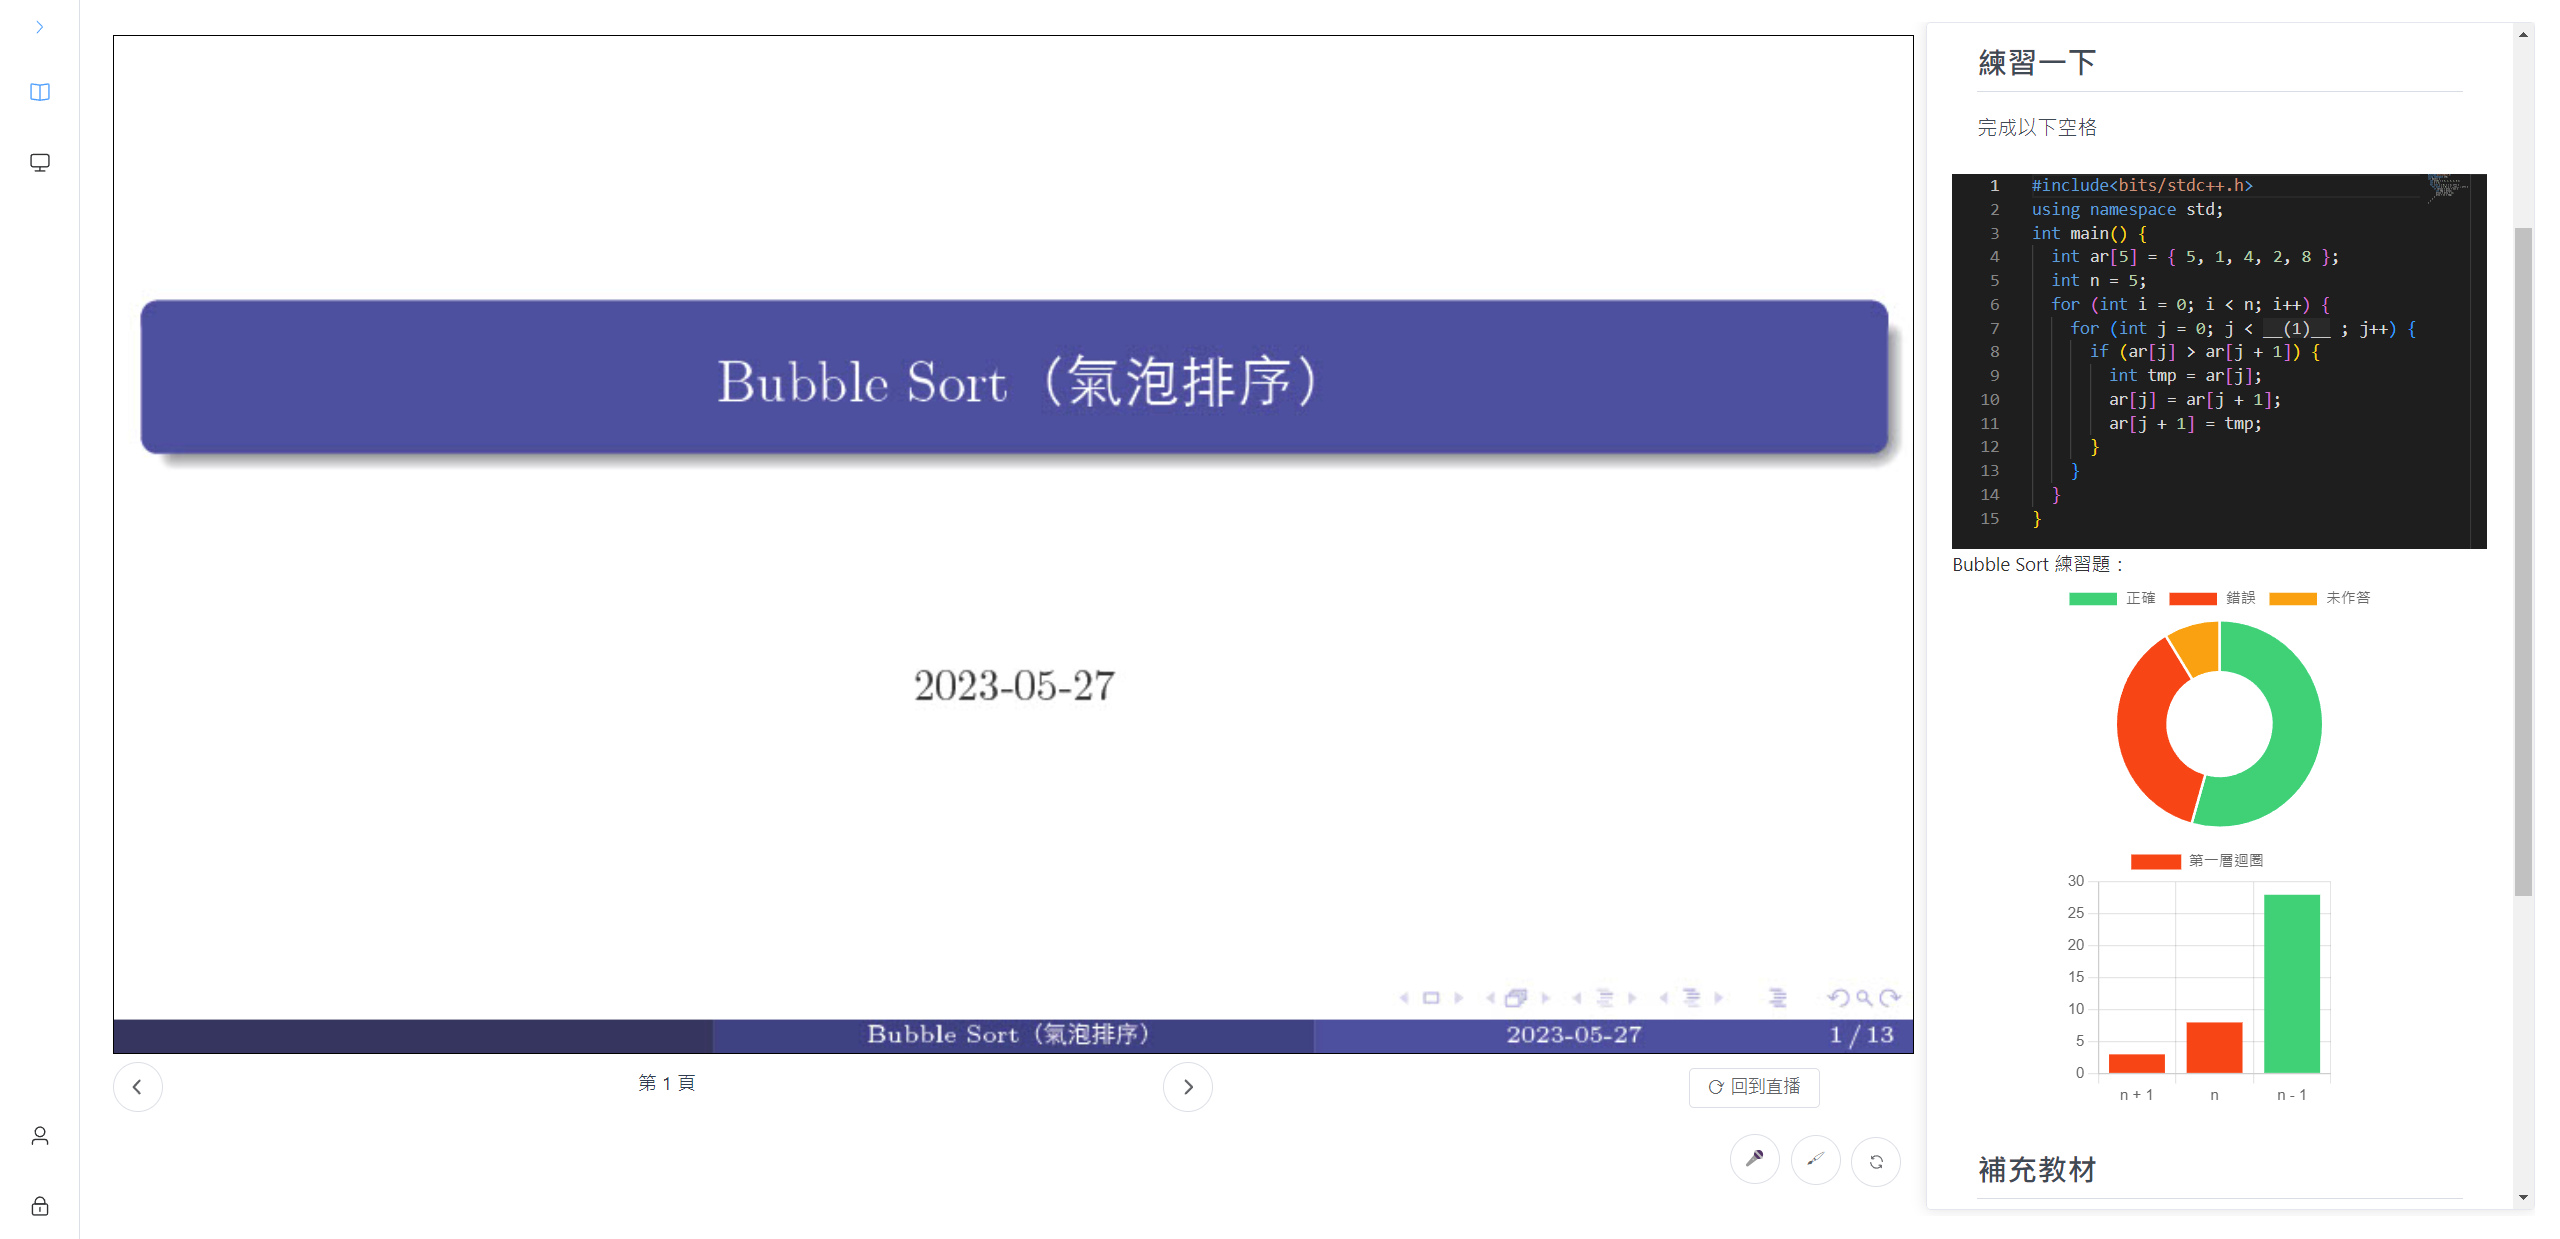
\includegraphics[width=1\textwidth]{images/teacher.png}
        % }
    \caption{教師課堂頁面}
  \end{subfigure}
  \caption{課堂介面}
  \label{fig:Classroom}
\end{figure}

% \subsubsection{產品的主要介面}

% \begin{enumerate}
%   \setlength{\parindent}{2em}

%   \item 學生課堂頁面:學生的課堂頁面有直播區、互動區、功能區
%   \begin{itemize}
%     \item 直播區:位於頁面左上用於顯示章節投影片,會在課中展示與老師相同的投影片畫面,並同步老師的滑鼠軌跡、繪畫等。
%     \item 互動區:位於頁面右側用於顯示滾動式的講義,講義可以放文字、圖片、課堂習題,並且在課中具有引導功能,會根據老師目前的上課投影片,用黃色框線在講義中顯示其對應的位置。
%     \item 功能區:位於頁面左下用於控制直播區的內容,在課中能夠切換投影片、一鍵回到老師的直播投影片等(圖\ref{fig:student-inClass}紅色框線處)。在課後能夠拖動時間軸,回放過去的上課直播(圖\ref{fig:student-review}紅色框線處)。
%   \end{itemize}

%   \begin{figure}[H]
%     \begin{subfigure}{0.5\linewidth}
%       \centering
%       %   \href{https://raw.githubusercontent.com/programingtw/proglearn-plan/main/img/student.png}{ 
%       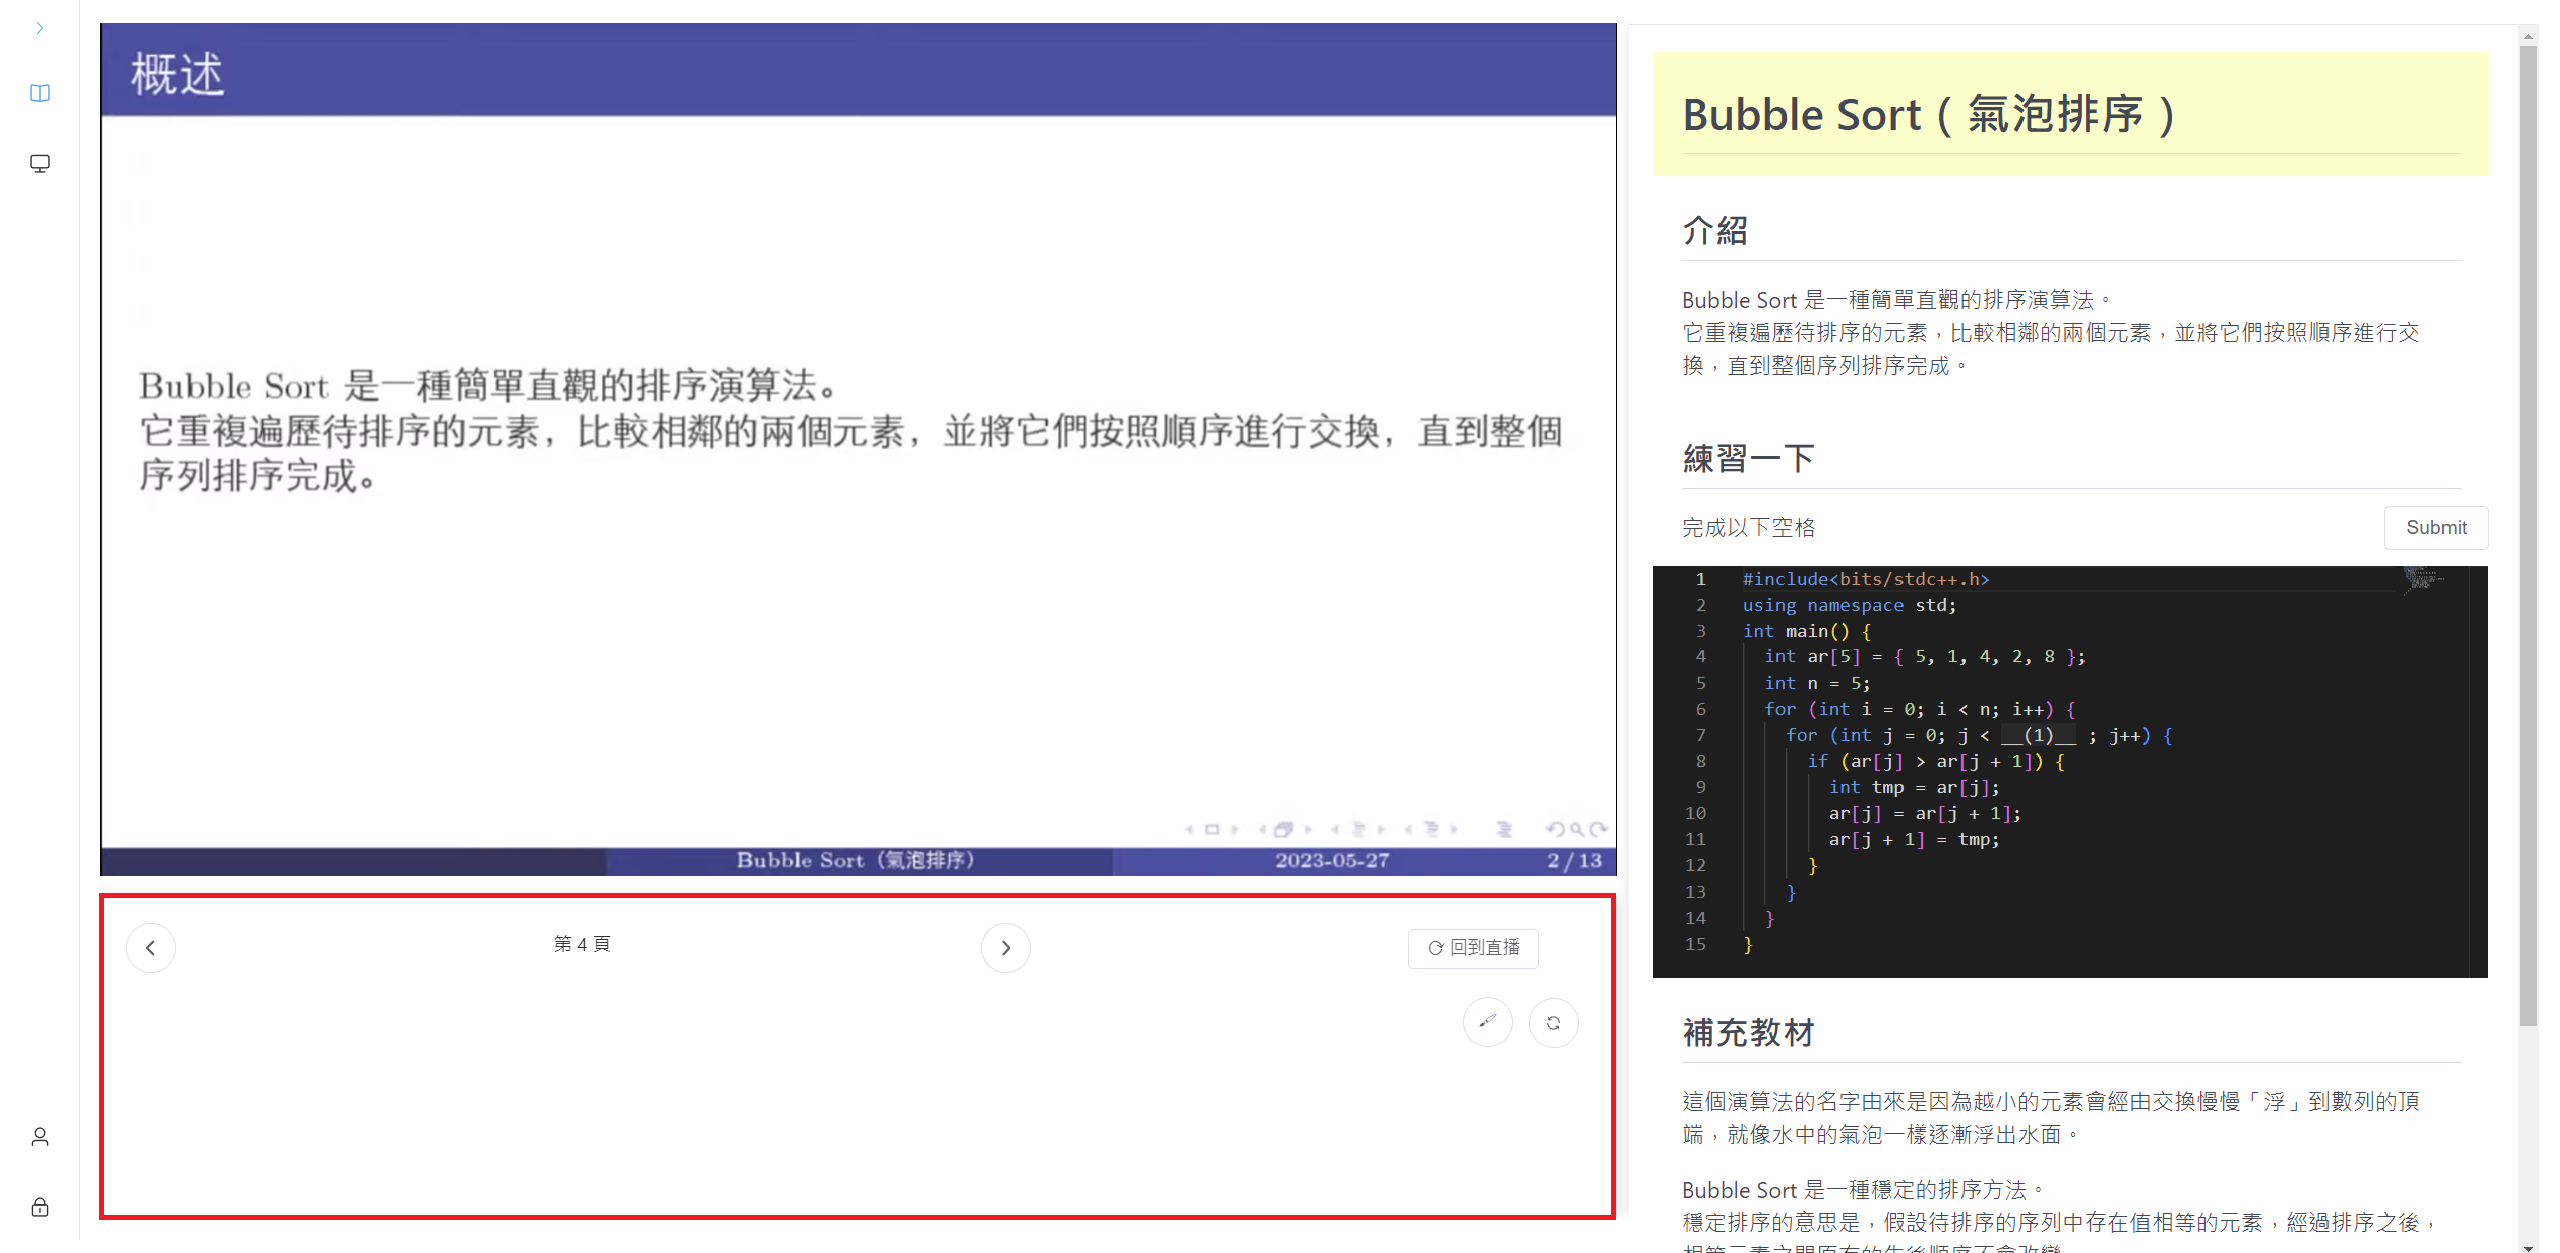
\includegraphics[width=1\textwidth]{images/student-In class.png}
%       %   }
%       \caption{學生課堂中}
%       \label{fig:student-inClass}
%     \end{subfigure}
%     \begin{subfigure}{0.5\linewidth}
%       \centering
%       %   \href{https://raw.githubusercontent.com/programingtw/proglearn-plan/main/img/teacher.png}{ 
%       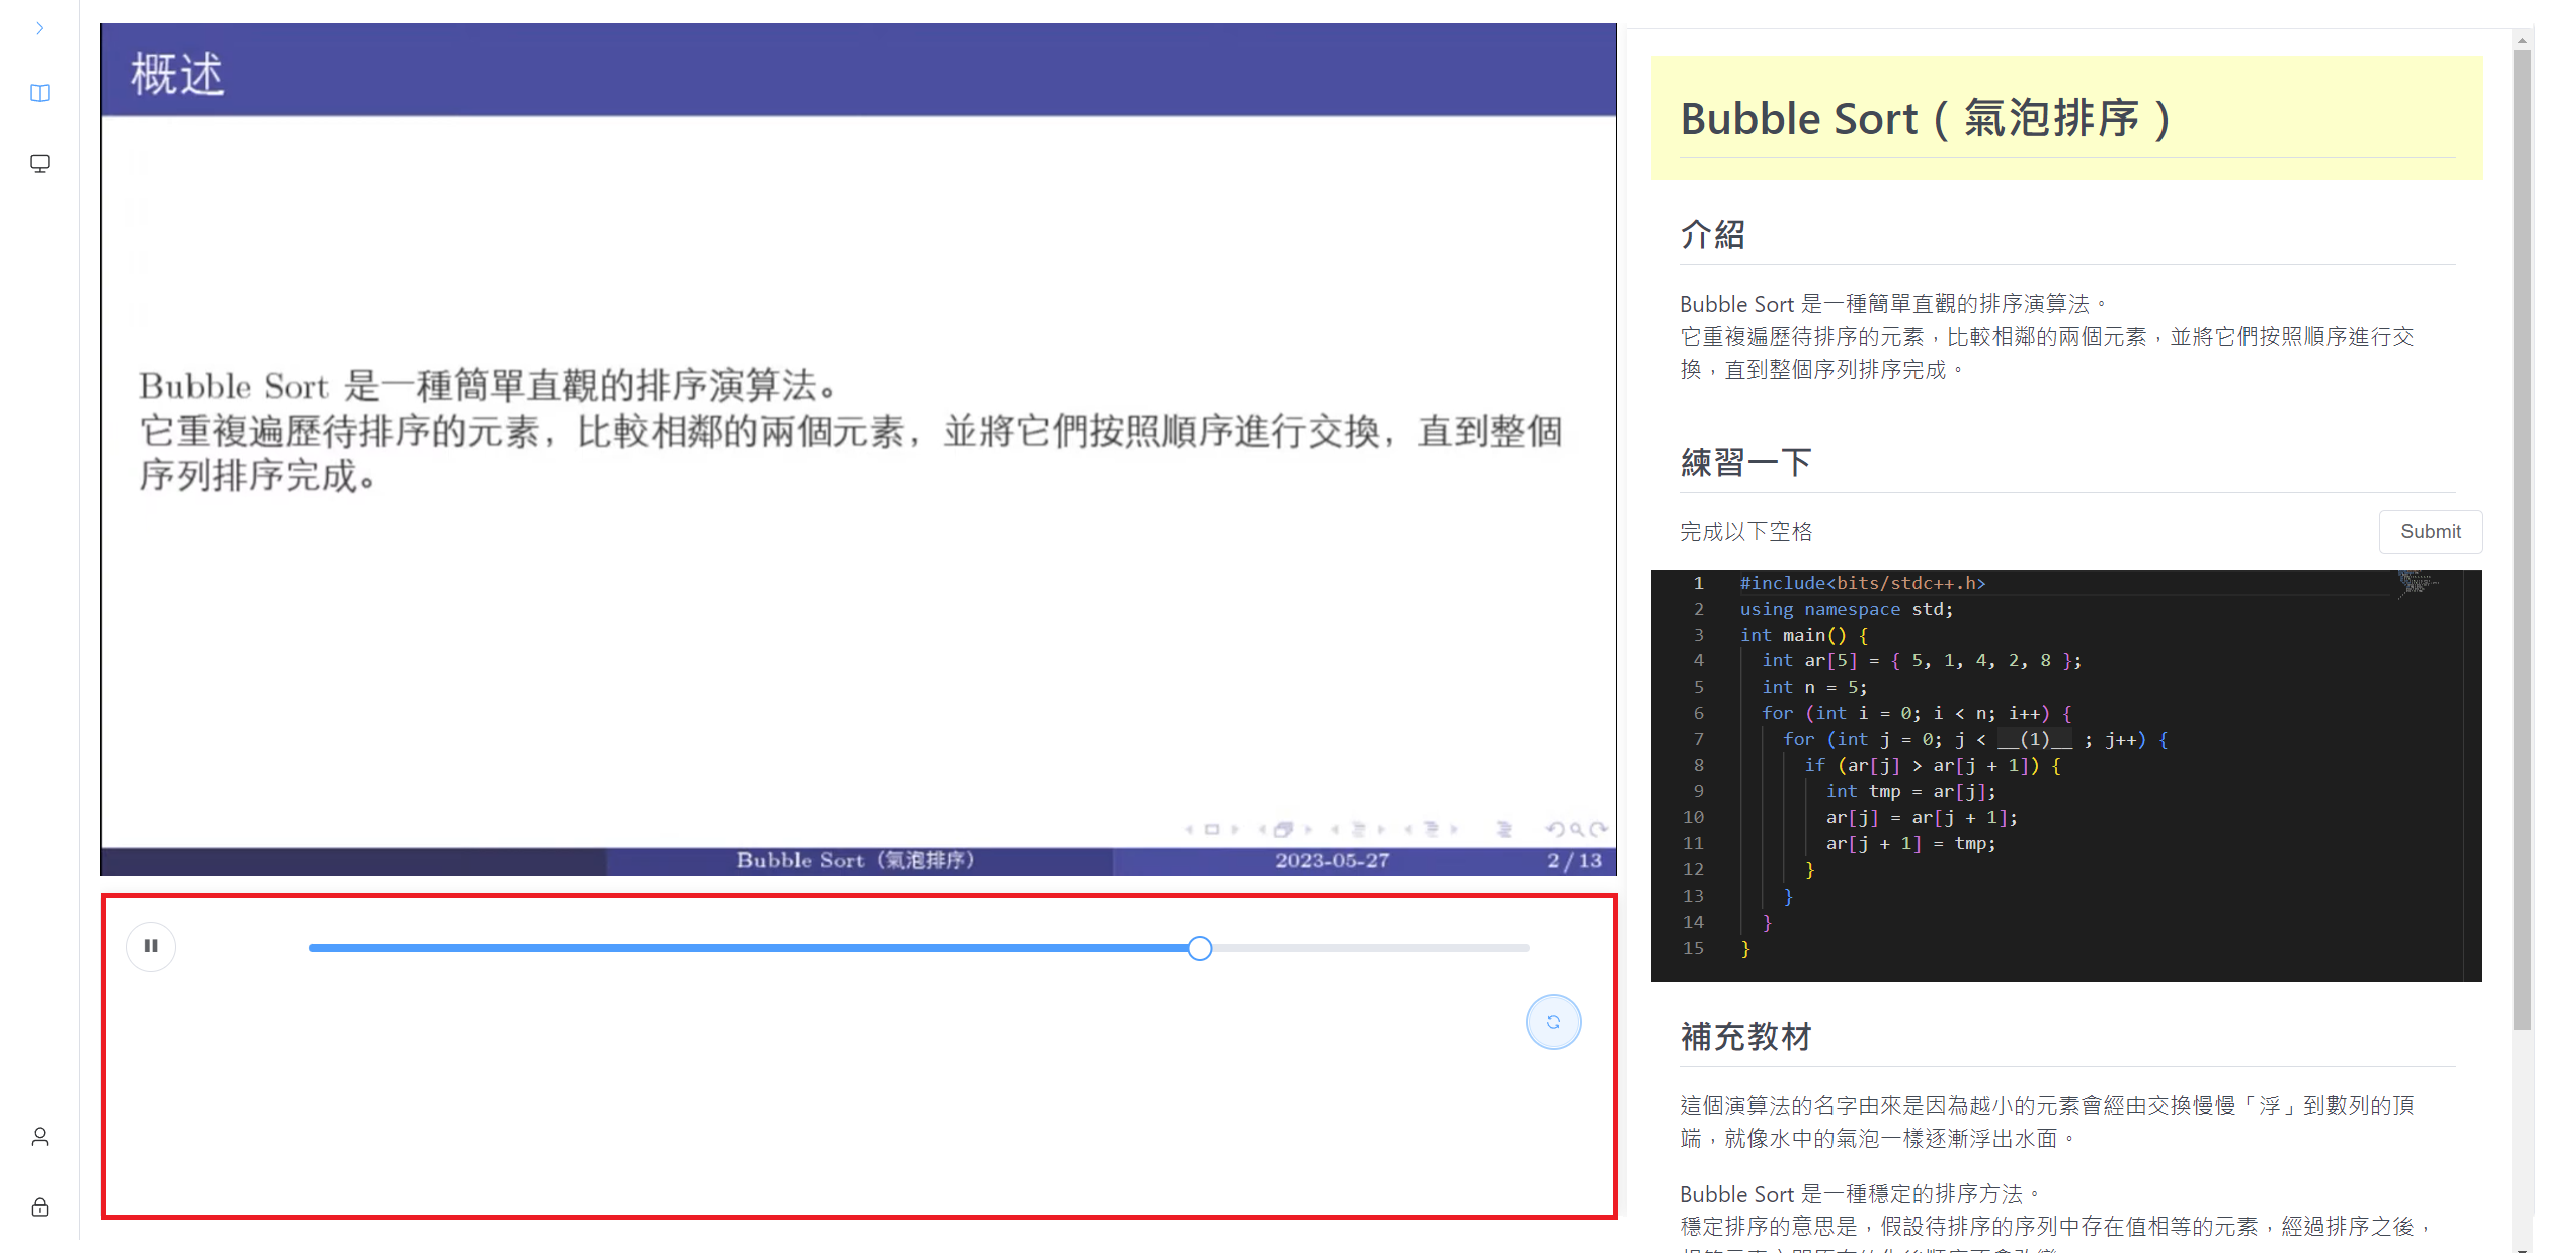
\includegraphics[width=1\textwidth]{images/review.png}
%       %   }
%       \caption{學生課後回放}
%       \label{fig:student-review}
%     \end{subfigure}
%     \caption{學生課堂頁面}
%   \end{figure}

%   \item 教師課堂頁面:教師的課堂頁面與學生的課堂頁面相同,同樣有直播區、互動區、功能區,但功能有部分差異。
%   \begin{itemize}
%     \item 直播區:位於頁面左上用於顯示章節投影片,在課中會將畫面同步到學生的直播區中。
%     \item 互動區:位於頁面右側用於顯示滾動式講義,並能夠預覽課堂習題的作答統計。
%     \item 功能區:位於頁面左下用於控制直播功能,能夠開啟與關閉直播,在課中可以切換投影片、切換成畫筆、開啟或關閉麥克風功能等。
%   \end{itemize}

%   \begin{figure}[H]
%     \centering
%     %   \href{https://raw.githubusercontent.com/programingtw/proglearn-plan/main/img/teacher.png}{ 
%     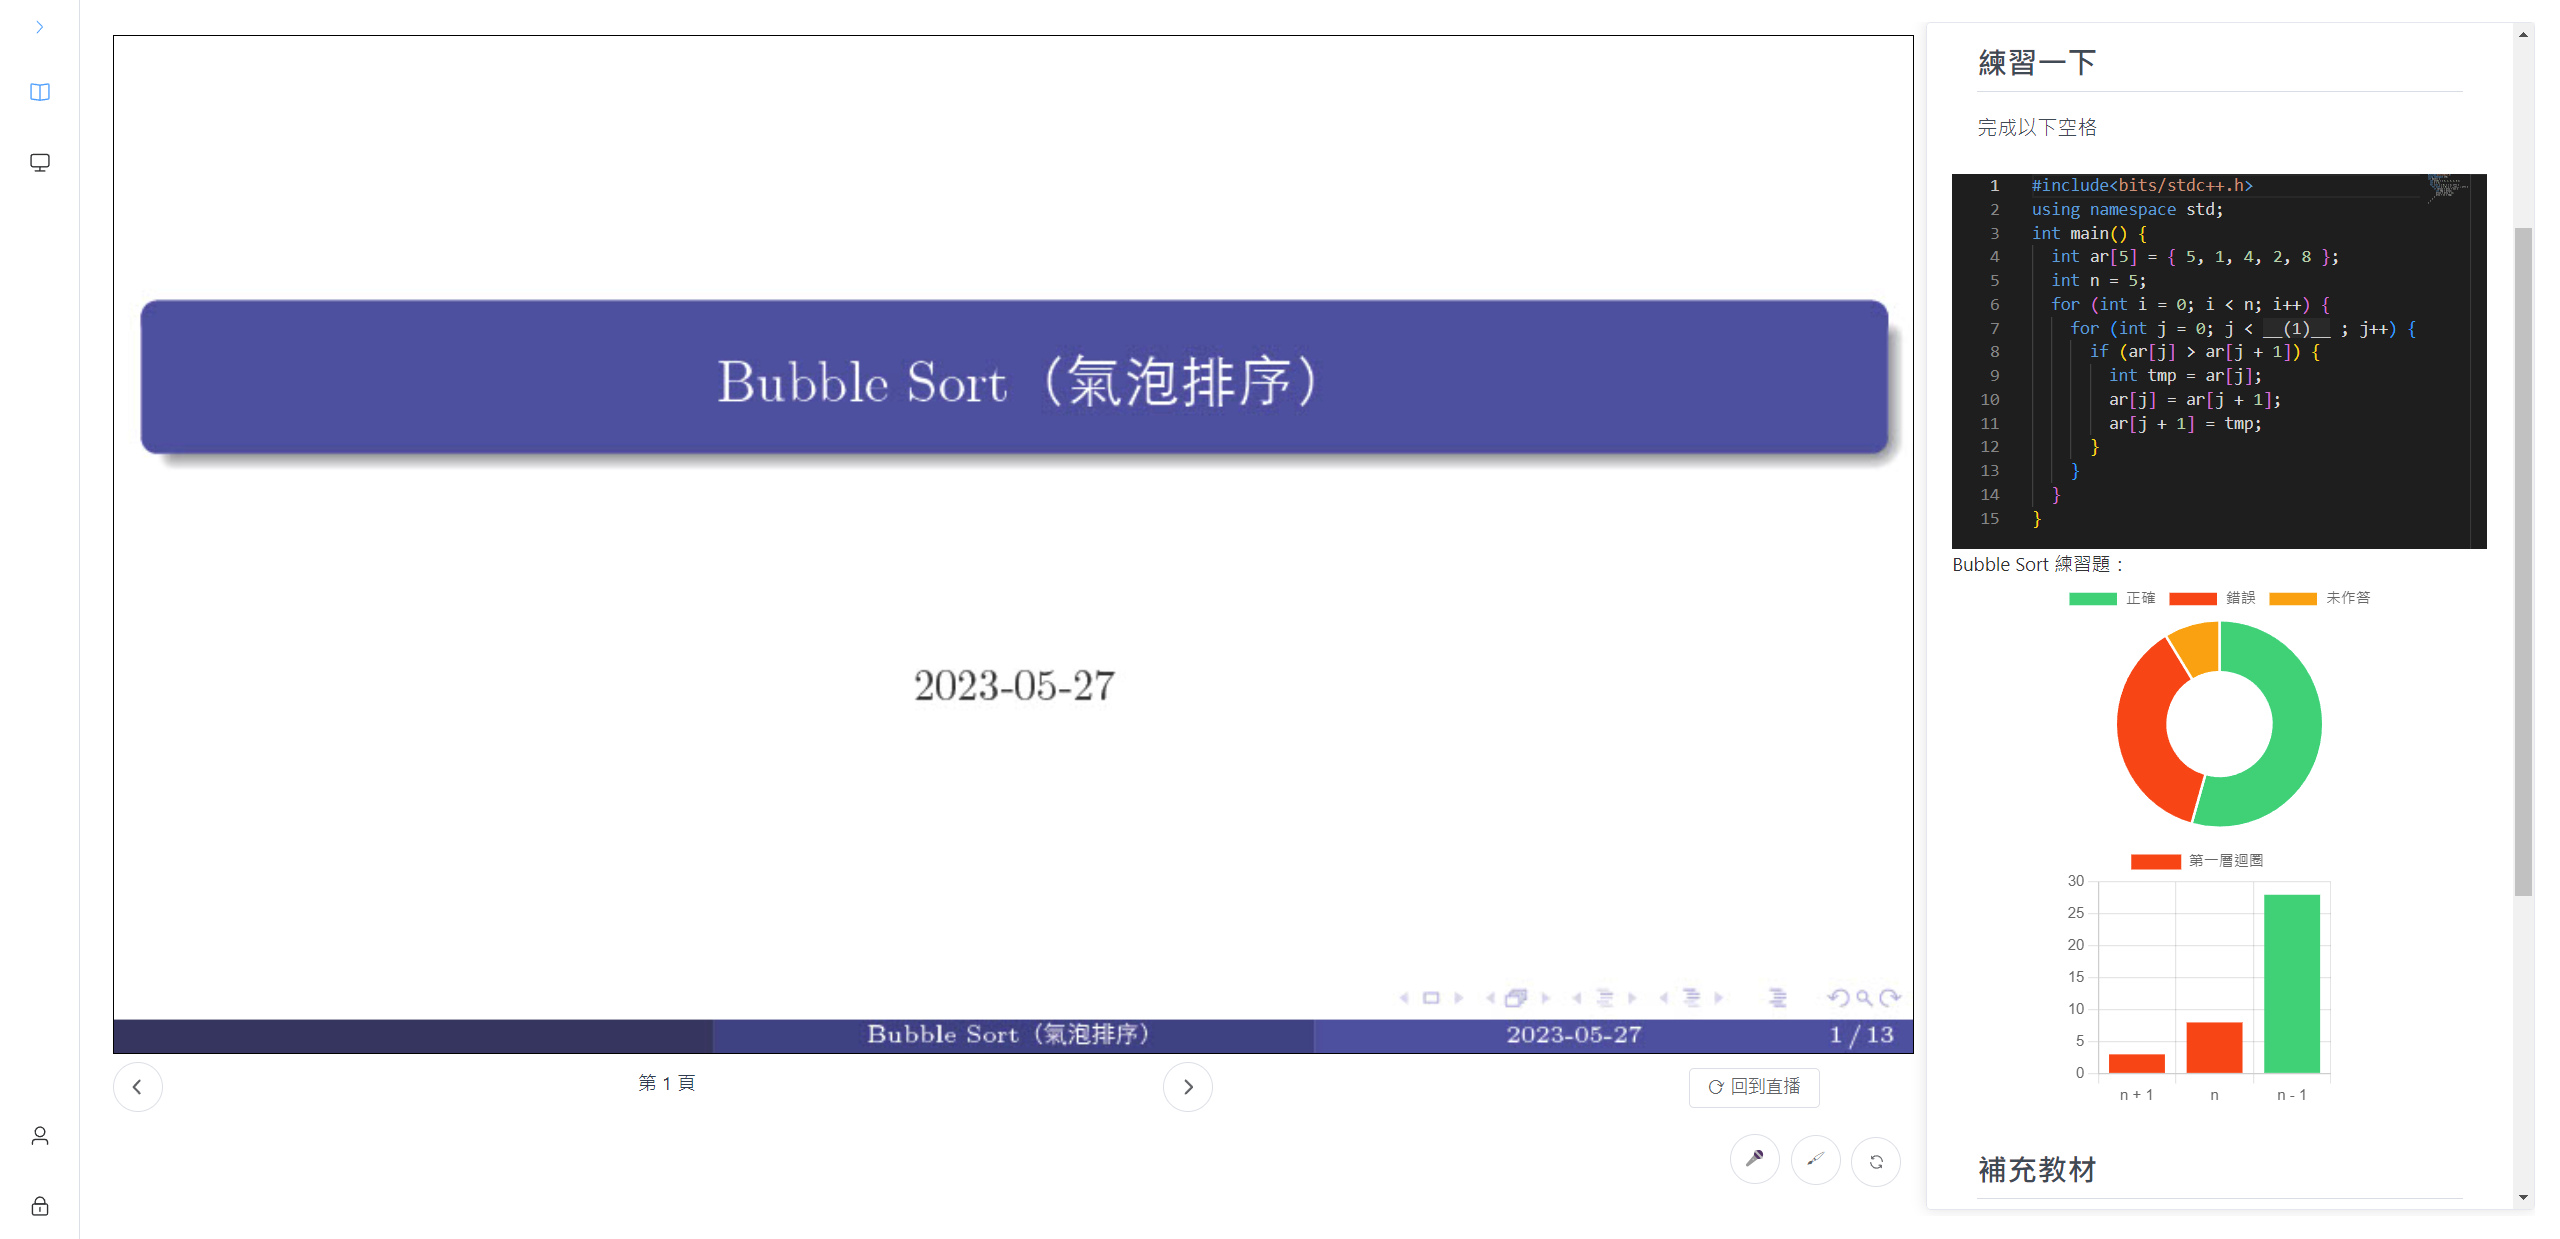
\includegraphics[width=0.7\textwidth]{images/teacher.png}
%     %   }
%     \caption{教師課堂頁面}
%   \end{figure}

%   \item 講義編輯頁面:教師可以在該頁面編輯講義的內容,並且將講義的不同部分組合成完整的講義內容(圖\ref{fig:edit-flowchart})。
%   \begin{itemize}
%     \item 編輯區:在右上點擊不同類型的講義區塊,如文字、選擇題、程式題,就能夠在左上編輯其中的內容。
%     \item 腳本區:下半部的時間軸,用於擺放不同類型的講義小區塊。時間軸的單位是投影片的頁數,讓投影片能對應到不同的講義區塊,在課中就能根據投影片的頁數在講義上做引導與提示。
%   \end{itemize}
%   \begin{figure}[H]
%     \centering
%     %   \href{https://raw.githubusercontent.com/programingtw/proglearn-plan/main/img/course.png}{ 
%     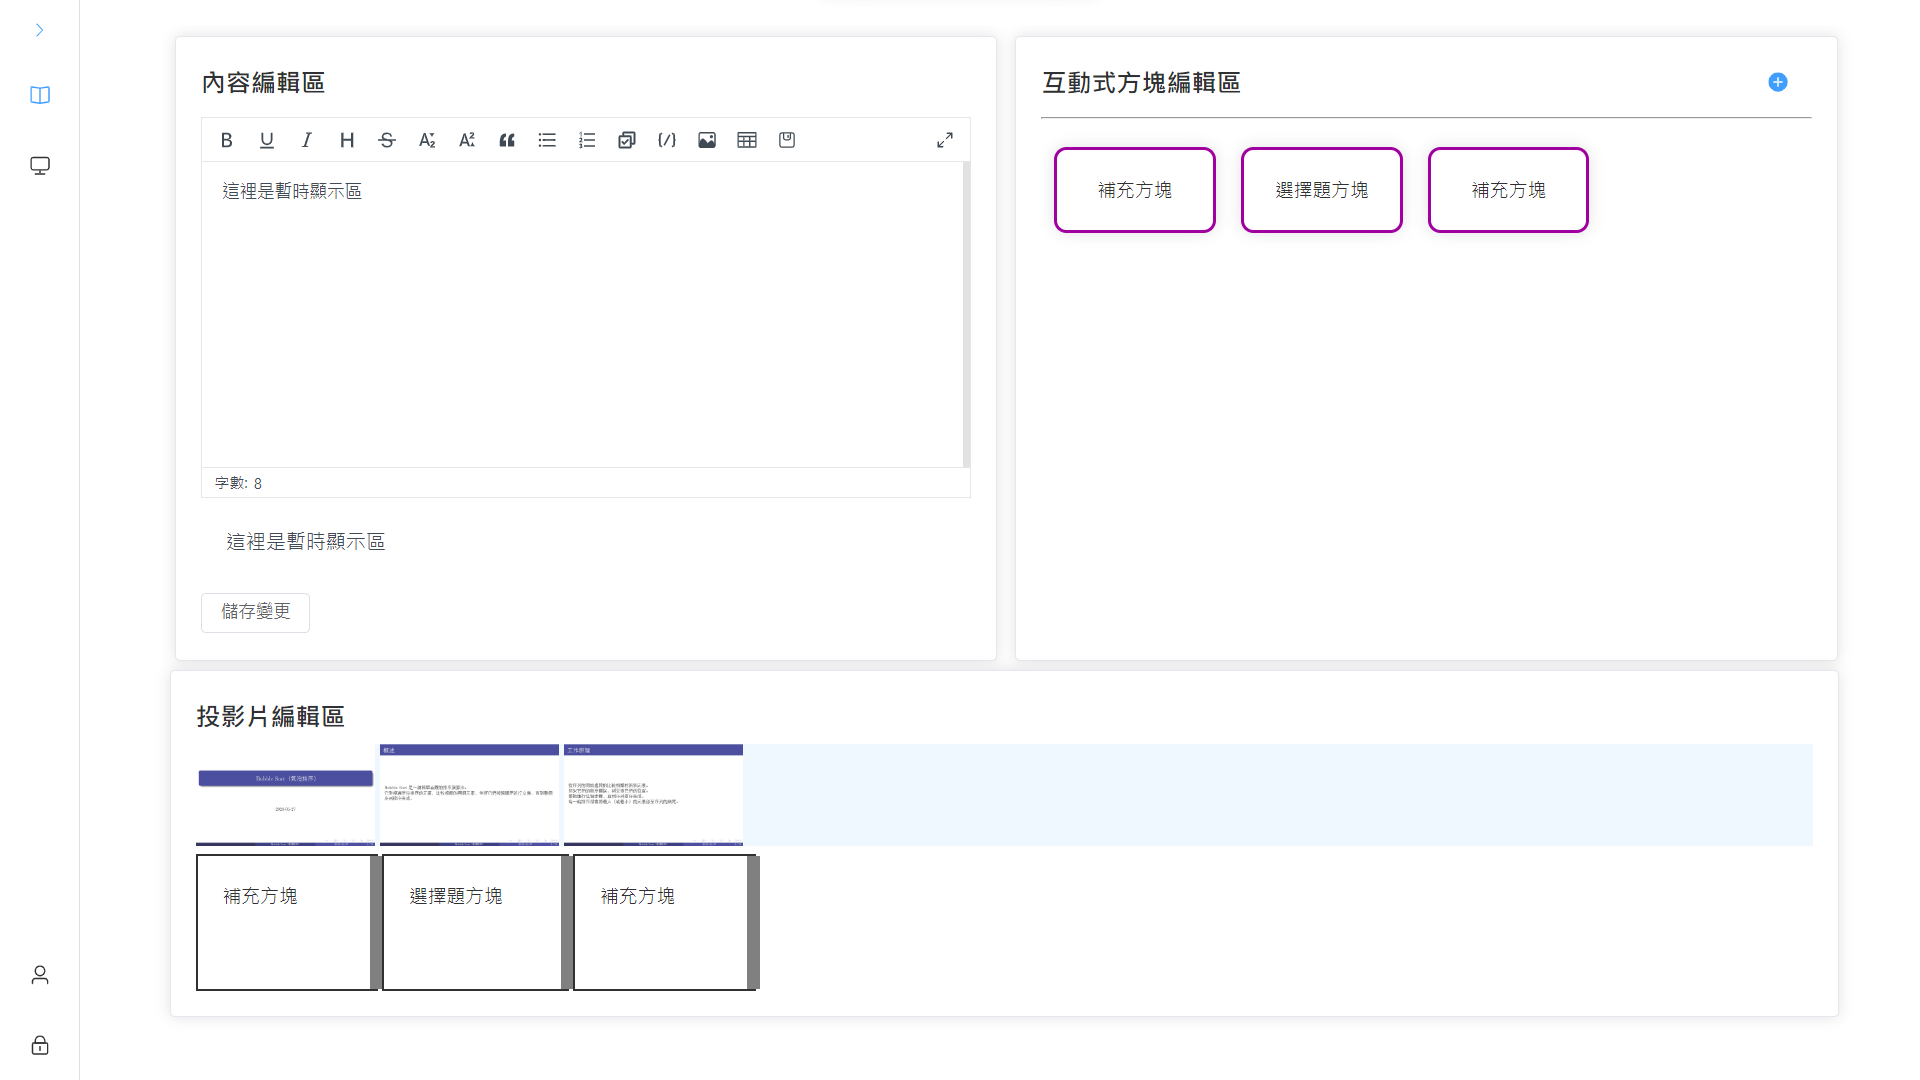
\includegraphics[width=0.7\textwidth]{images/edit.png}
%     %   }
%     \caption{講義編輯頁面}
%   \end{figure}

%   \begin{figure}[H]
%     \centering
%     \begin{tikzpicture}[node distance=4cm]
  
%       \node (start) [startstop] {點擊加號新增互動式方塊};
%       \node (pro1) [process, right of=start, xshift=2cm] {點擊互動式方塊};
%       \node (pro2) [process, right of=pro1] {編輯方塊內容};
%       \node (pro3) [process, below of=pro2] {儲存變更};
%       \node (pro4) [process, left of=pro3] {拖曳方塊到投影片};
%       \node (pro5) [process, left of=pro4] {調整方塊長度};
%       \node (stop) [startstop, left of=pro5] {完成講義編輯};
  
%       \draw [arrow] (start) -- (pro1);
%       \draw [arrow] (pro1) -- (pro2);
%       \draw [arrow] (pro2) -- (pro3);
%       \draw [arrow] (pro3) -- (pro4);
%       \draw [arrow] (pro4) -- (pro5);
%       \draw [arrow] (pro5) -- (stop);
  
%     \end{tikzpicture}
%     \caption{講義編輯的使用流程圖}
%     \label{fig:edit-flowchart}
%   \end{figure}

% \end{enumerate}

\subsubsection{直播功能(低延遲串流)}

\begin{figure}[H]
  \centering
  %   \href{https://raw.githubusercontent.com/programingtw/proglearn-plan/main/img/live.png}{ 
  
\includegraphics[width=0.5\textwidth]{images/streaming.png}
  %   }
  \caption{直播功能區}
\end{figure}

直播功能區位在課堂介面的左半部。此直播功能不同於往常的影像傳輸,而是記錄教師在投影片上的所有操作,包含換頁、繪畫、游標軌跡和聲音實時同步到學生端的介面上,然後存儲在直播記錄中,方便回顧與學習。
因此相比於Zoom、Meet等視訊會議工具,具有更低的網路延遲與頻寬需求,並且更加穩定。



% \begin{figure}[H]
%   \centering
%   \begin{tikzpicture}[node distance=4cm]

%     \node (start) [startstop] {教師移動滑鼠游標};
%     \node (pro1) [process, right of=start, xshift=1cm] {將滑鼠移動資訊傳到伺服器};
%     \node (pro2) [process, right of=pro1, xshift=2cm] {伺服器儲存至直播記錄};
%     \node (pro3) [process, below of=pro2, yshift=2cm] {伺服器將資訊傳到學生端};
%     \node (stop) [process, left of=pro3, xshift=-2cm] {學生端顯示滑鼠游標軌跡};
%     \draw [arrow] (start) -- (pro1);
%     \draw [arrow] (pro1) -- (pro2);
%     \draw [arrow] (pro2) -- (pro3);
%     \draw [arrow] (pro3) -- (stop);

%   \end{tikzpicture}
%   \caption{直播的傳輸流程圖}
%   \label{fig:streaming-flowchart}
% \end{figure}

% 由於其低延遲的特性,可以讓教師在即時的課堂環境中使用,作為教學的輔助工具。在線上與偏鄉教學中,其更低的硬體需求,可以作為主要的教學工具。

% 此外,該直播系統是基於投影片的直播,因此學生可以在課堂中自由地回顧投影片的內容,並且可以在課後自由地拖動時間軸,回放過去的上課直播。

\subsubsection{互動式講義}

\begin{figure}[H]
  \begin{subfigure}{0.5\linewidth}
    \centering
    %   \href{https://raw.githubusercontent.com/programingtw/proglearn-plan/main/img/student.png}{ 
    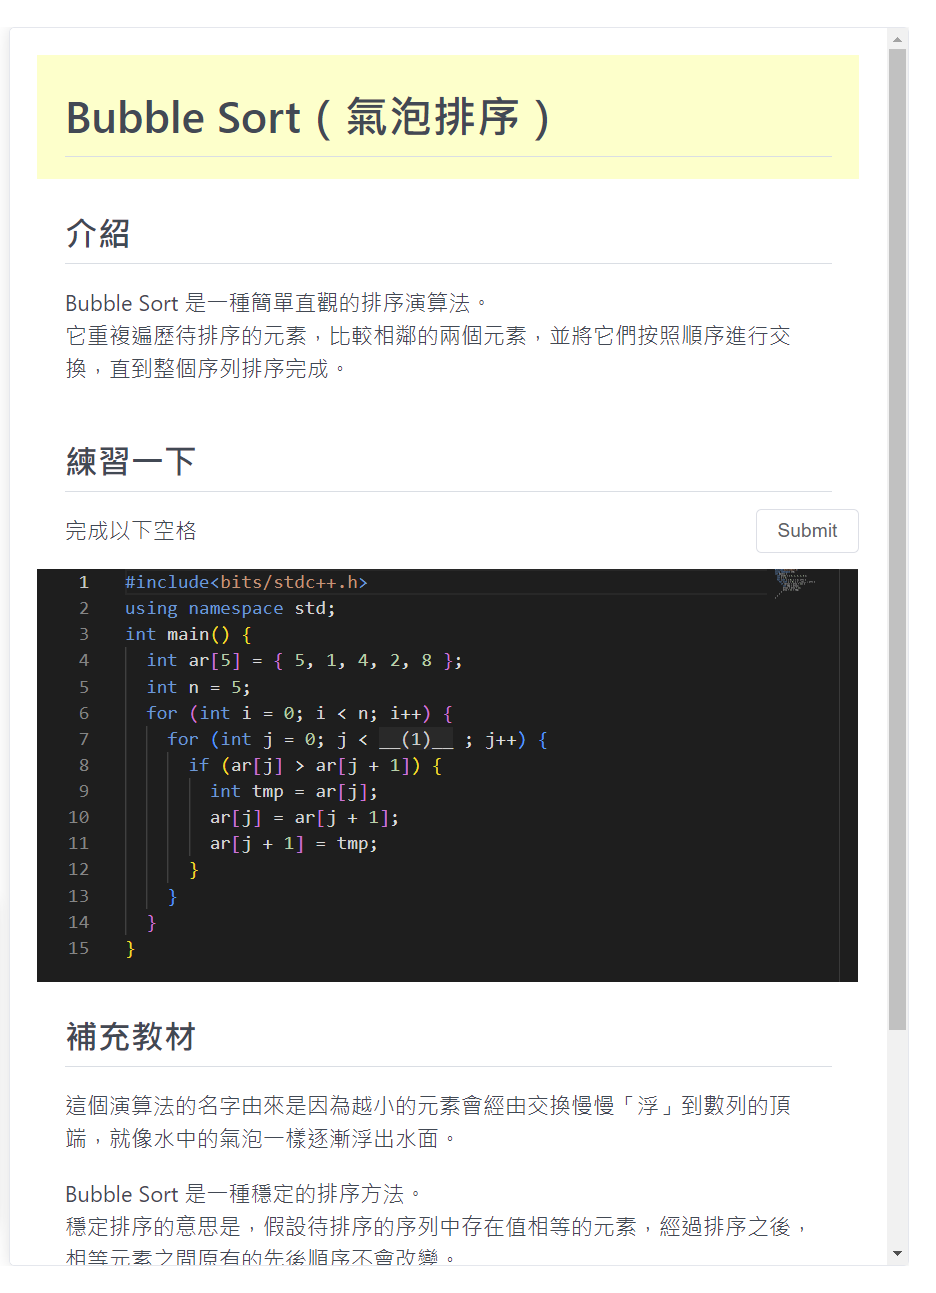
\includegraphics[width=0.6\textwidth]{images/side-s.png}
    %   }
    \caption{學生講義頁面}
    \label{fig:student}
  \end{subfigure}
  \begin{subfigure}{0.5\linewidth}
    \centering
        % \href{https://raw.githubusercontent.com/programingtw/proglearn-plan/main/img/teacher.png}{ 
    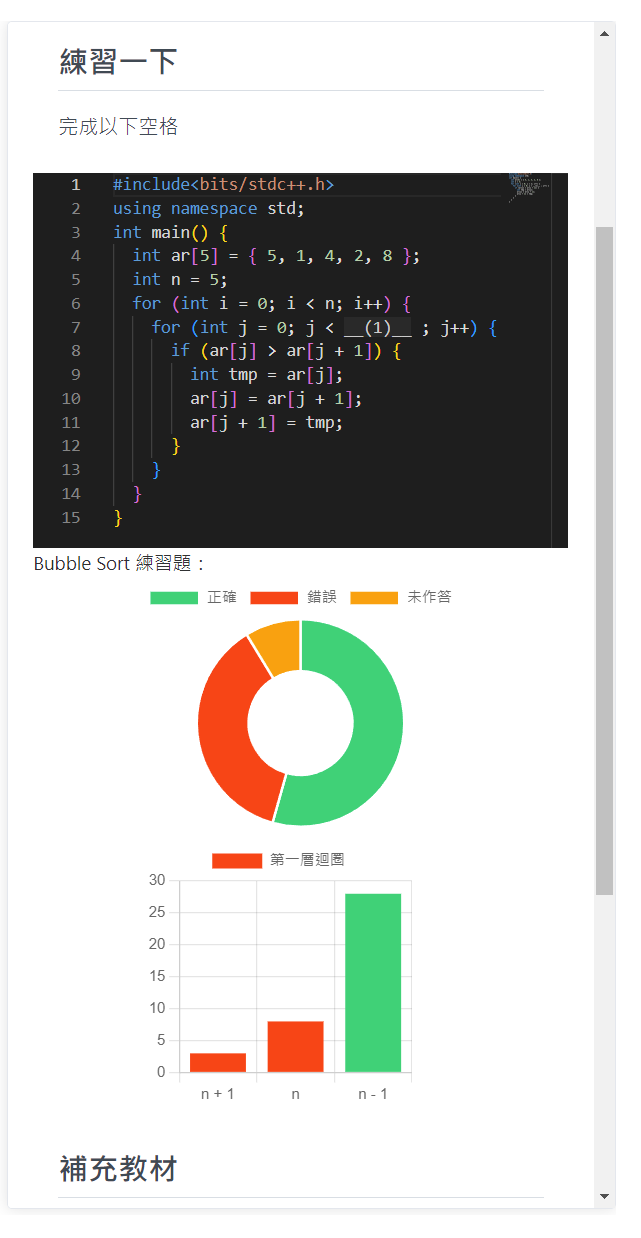
\includegraphics[width=0.45\textwidth]{images/side-t.png}
        % }
    \caption{教師講義頁面}
    \label{fig:teacher}
  \end{subfigure}
  \caption{互動式講義區塊}
\end{figure}

互動式講義位在課堂介面的右半部。目的是在課堂中能提供師生間互動的橋樑,並作為教學與學習的輔助工具。其相關功能可細分為以下四點:

\begin{enumerate}
  \setlength{\parindent}{2em}

  \item 智慧引導
  \par 透過淺黃色區塊,向學生指引出當前的投影片對應到講義上的哪些部分(圖\ref{fig:student})。
  
  \item 即時反饋(數位儀表板)
  \par 為教師提供學生的課堂作答情況,即時了解學生的學習狀況(圖\ref{fig:teacher}下半部)。

  \item 自動批改
  \par 為學生提供課堂上的程式作答功能,其使用流程可參考圖\ref{fig:problem-flowchart}。該功能可以自動並即時批改課堂習題,並且在教師的數位儀表板上顯示學生的作答情況(圖\ref{fig:teacher})。其技術也應用於作業管理中(\ref{sec:course-assignment}節)。
  
  \begin{figure}[H]
    \centering
    \begin{tikzpicture}[node distance=4cm]
  
      \node (start) [startstop] {學生撰寫程式習題};
      \node (pro1) [process, right of=start, xshift=1cm] {學生點擊submit(圖\ref{fig:student})};
      \node (pro2) [process, right of=pro1, xshift=1cm] {顯示作答結果};
      \node (pro3) [process, below of=pro2, yshift=2cm] {教師課堂頁面更新};
      \node (stop) [process, left of=pro3, xshift=-2cm] {數位儀表板顯示作答統計(圖\ref{fig:teacher})};
  
      \draw [arrow] (start) -- (pro1);
      \draw [arrow] (pro1) -- (pro2);
      \draw [arrow] (pro2) -- (pro3);
      \draw [arrow] (pro3) -- (stop);
  
    \end{tikzpicture}
    \caption{程式作答的使用流程圖}
    \label{fig:problem-flowchart}
  \end{figure}

  \item 講義視覺化編輯
  \par 講義編輯頁面為教師提供編輯講義的功能(圖\ref{fig:edit}左半部)。在編排講義時,教師可以對不同的講義物件做編輯,包括選擇題方塊、補充方塊等,然後將該物件拖曳到時間軸中,組合成一個完整的講義(圖\ref{fig:edit}右半部)。而在時間軸中將一一對應著投影片的頁數,因此在課堂中,當老師切換到特定的頁數時,就能在講義中標示出對應的上課內容(圖\ref{fig:student}的淺黃色區塊)。

  % \begin{figure}[H]
  %   \begin{subfigure}{0.5\linewidth}
  %     \centering
  %     %   \href{https://raw.githubusercontent.com/programingtw/proglearn-plan/main/img/course.png}{ 
  %     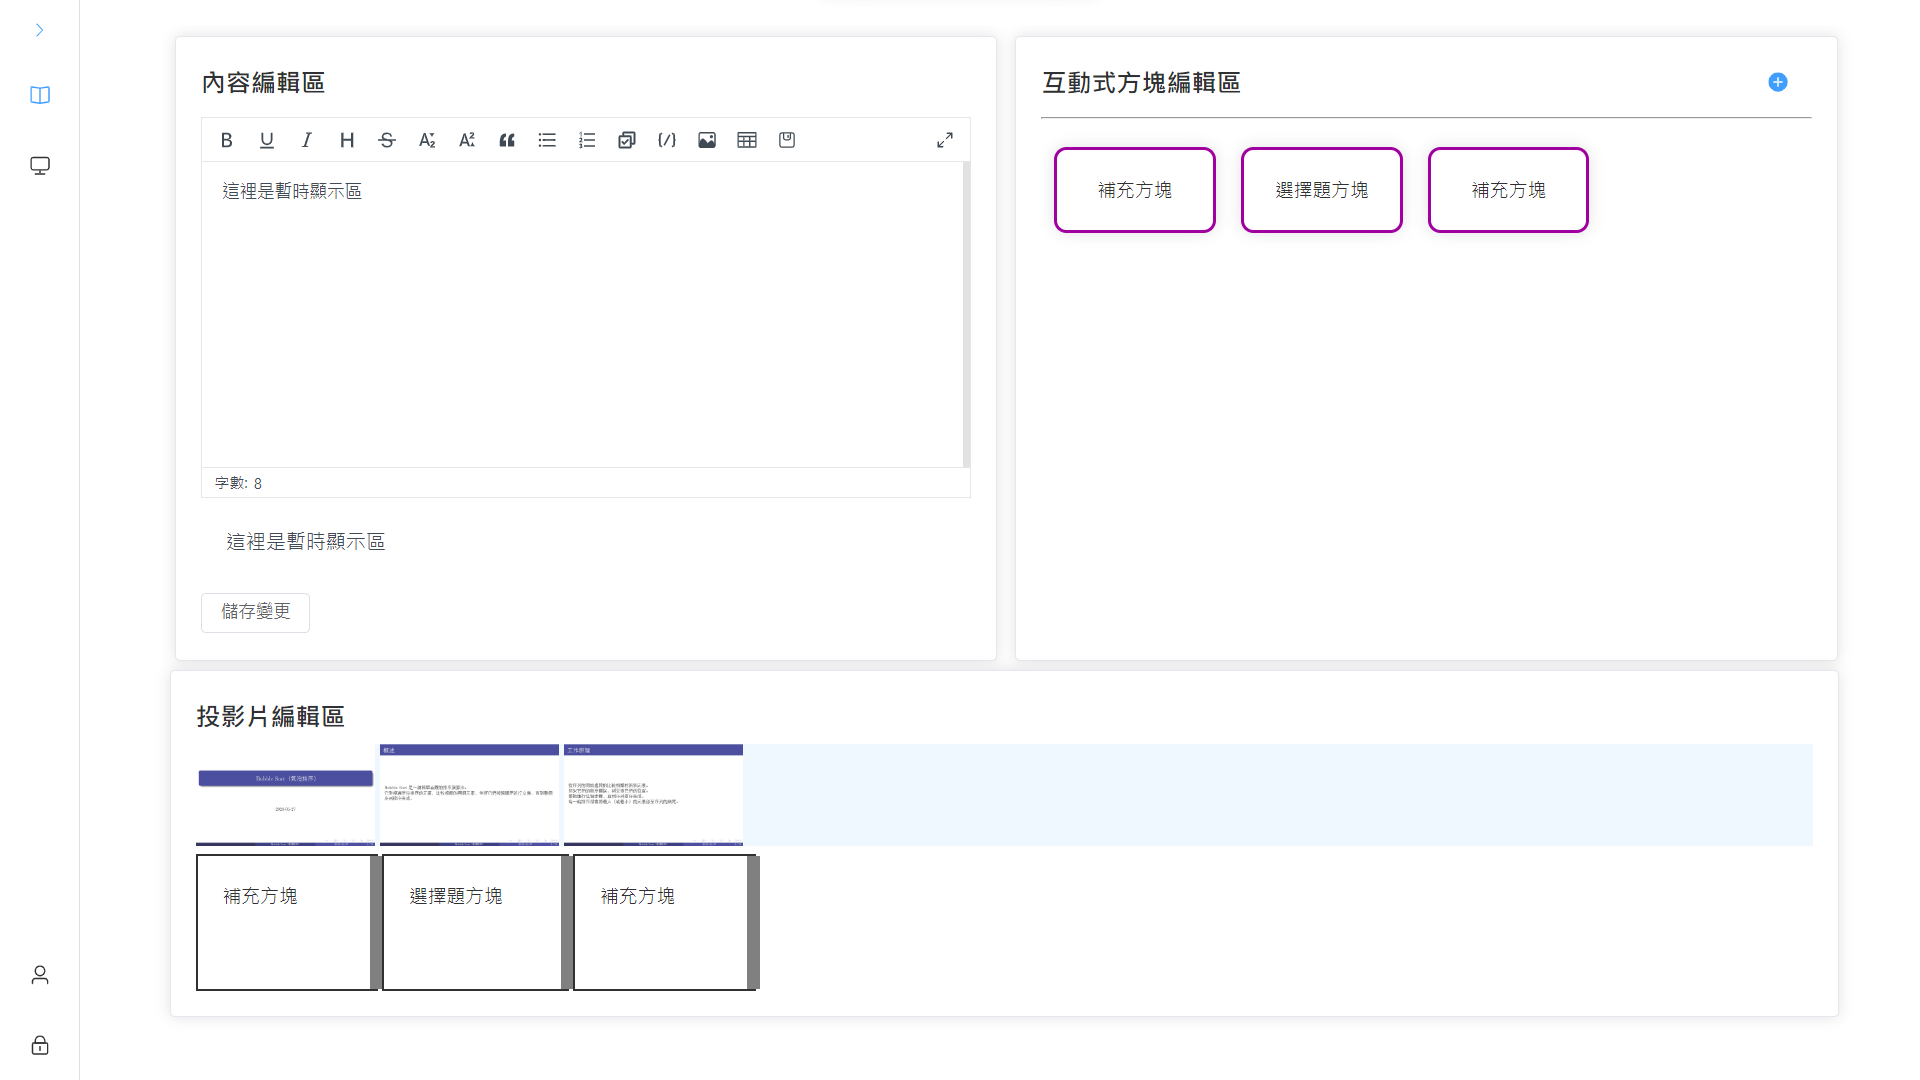
\includegraphics[width=1\textwidth]{images/edit.png}
  %     %   }
  %     \caption{講義編輯頁面}
  %     \label{fig:edit}
  %   \end{subfigure}
  %   \begin{subfigure}{0.5\linewidth}
  %     \centering
  %     %   \href{https://raw.githubusercontent.com/programingtw/proglearn-plan/main/img/list.png}{ 
  %     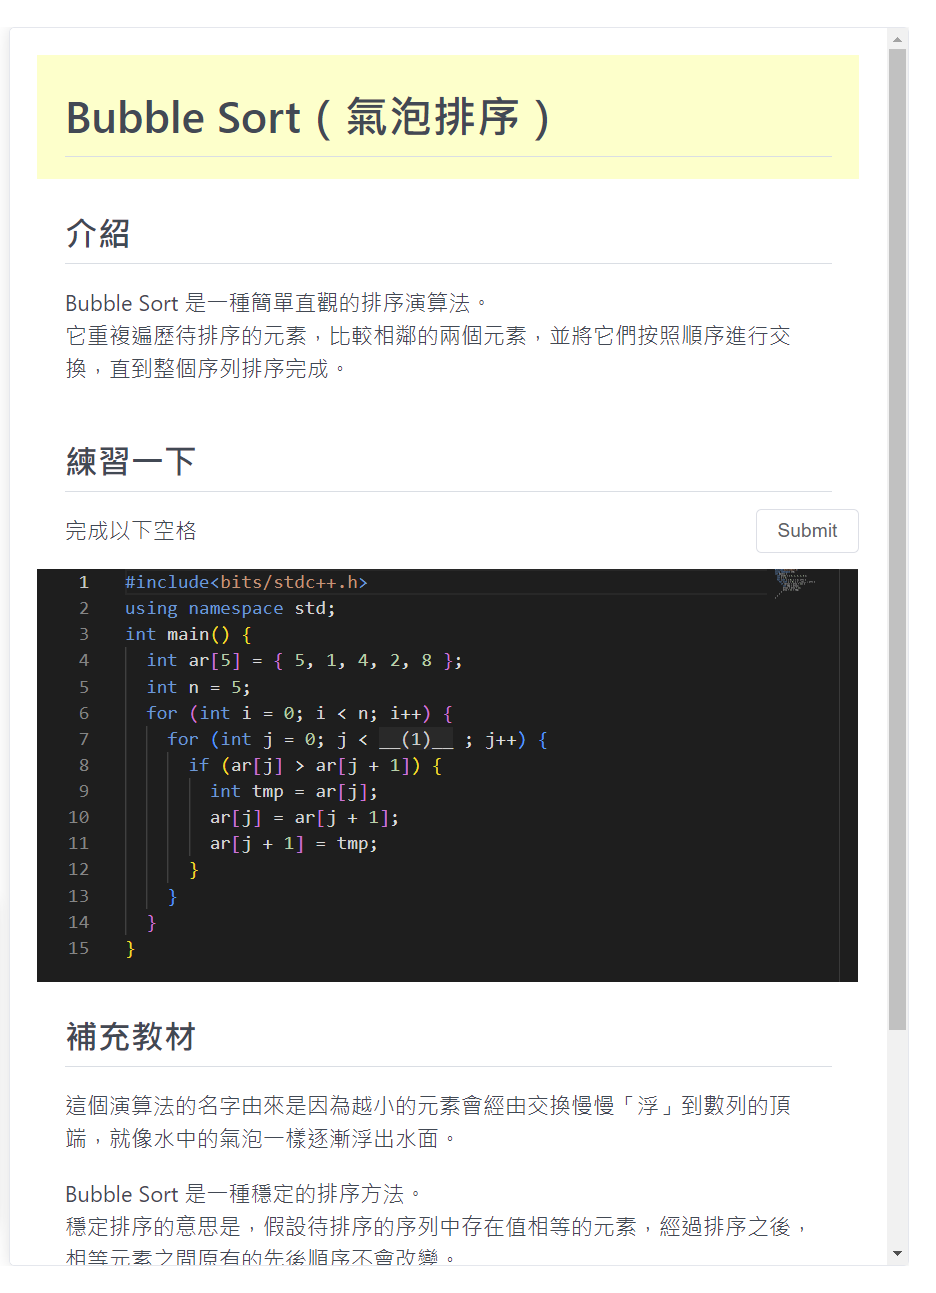
\includegraphics[width=0.5\textwidth]{images/side-s.png}
  %     %   }
  %     \caption{顯示的講義}
  %     \label{fig:textbook}
  %   \end{subfigure}
  %   \caption{講義編輯功能}
  % \end{figure}

  \begin{figure}[H]
    \centering
    %   \href{https://raw.githubusercontent.com/programingtw/proglearn-plan/main/img/live.png}{ 
    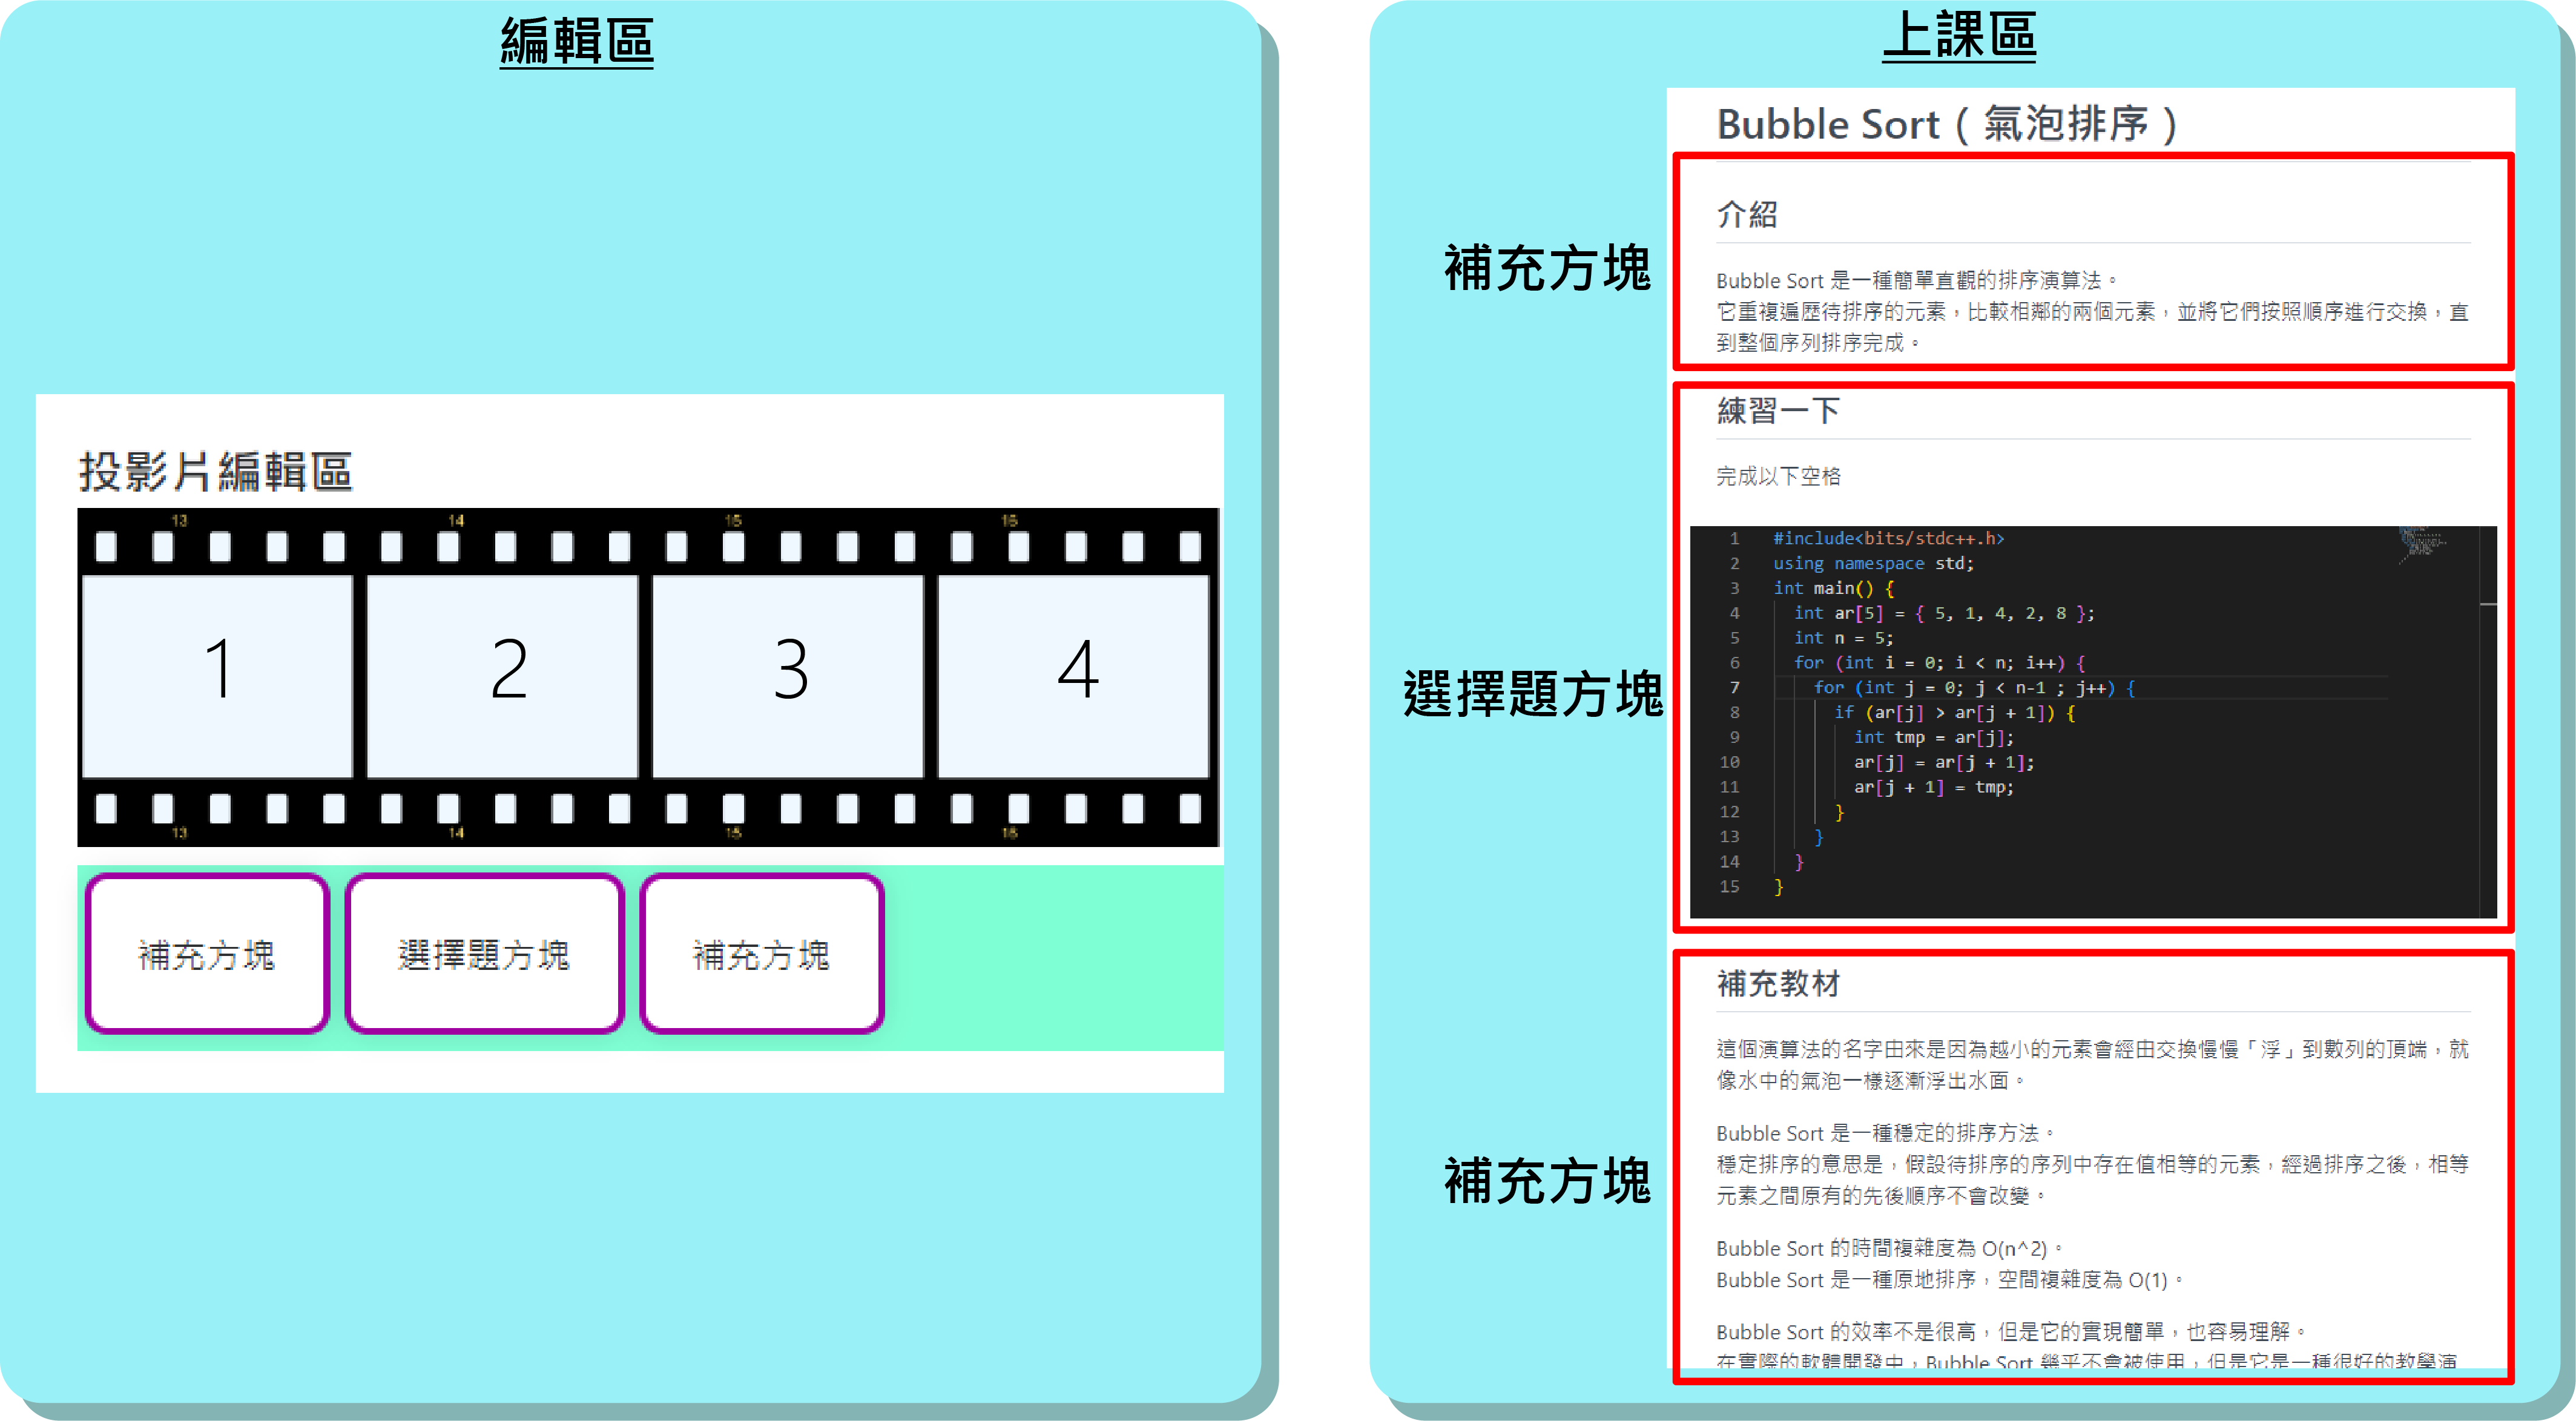
\includegraphics[width=0.8\textwidth]{images/timezone.png}
    %   }
    \caption{講義編輯的示意圖}
    \label{fig:edit}
  \end{figure}

\end{enumerate}

\subsubsection{課程與作業管理}
\label{sec:course-assignment}

本系統在課堂外,提供了課程與作業管理的功能。教師可以在此設定課程章節、作業、測驗、考試與查看學生作答狀況。學生可以在此查看課程資訊(圖\ref{fig:course})、撰寫作業(圖\ref{fig:homework})並得到即時批改(圖\ref{fig:course-assignment-flowchart})。

\begin{figure}[H]
    \centering
    \begin{tikzpicture}[node distance=2cm, auto]

      \node (start) [startstop] {教師設定課程作業};
      \node (pro1) [process, right of=start, xshift=3cm] {學生查看作業資訊};
      \node (pro2) [process, right of=pro1, xshift=3cm] {學生撰寫作業並送出};
      \node (pro3) [process, below of=pro2] {系統自動批改};
      \node (pro4) [process, left of=pro3, xshift=-3cm] {學生查看批改結果};
      \node (stop) [process, left of=pro4, xshift=-3cm] {教師查看作答統計};

      \draw [arrow] (start) -- (pro1);
      \draw [arrow] (pro1) -- (pro2);
      \draw [arrow] (pro2) -- (pro3);
      \draw [arrow] (pro3) -- (pro4);
      \draw [arrow] (pro4) -- (stop);

    \end{tikzpicture}
    \caption{作業管理系統流程圖}
    \label{fig:course-assignment-flowchart}
\end{figure}

\begin{figure}[H]
  \begin{subfigure}{0.5\linewidth}
    \centering
    %   \href{https://raw.githubusercontent.com/programingtw/proglearn-plan/main/img/list.png}{ 
    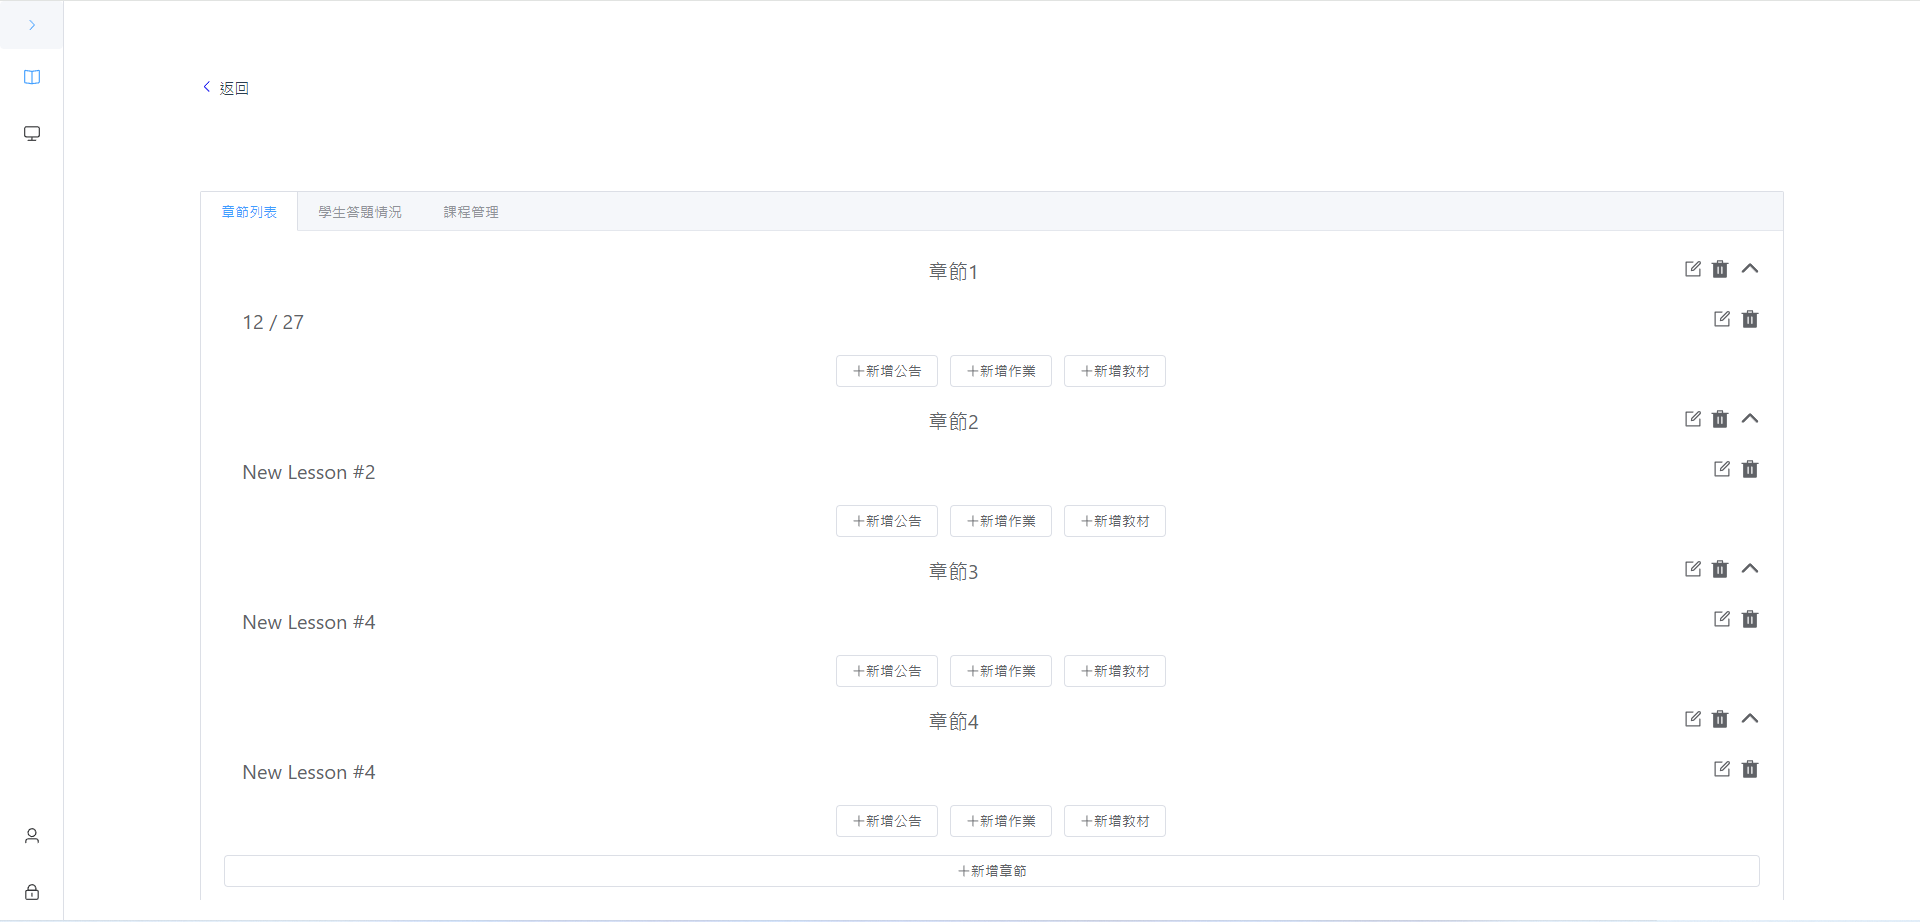
\includegraphics[width=0.75\textwidth]{images/chapter.png}
    %   }
    \caption{課程章節}
  \end{subfigure}
  \begin{subfigure}{0.5\linewidth}
    \centering
    %   \href{https://raw.githubusercontent.com/programingtw/proglearn-plan/main/img/course.png}{ 
    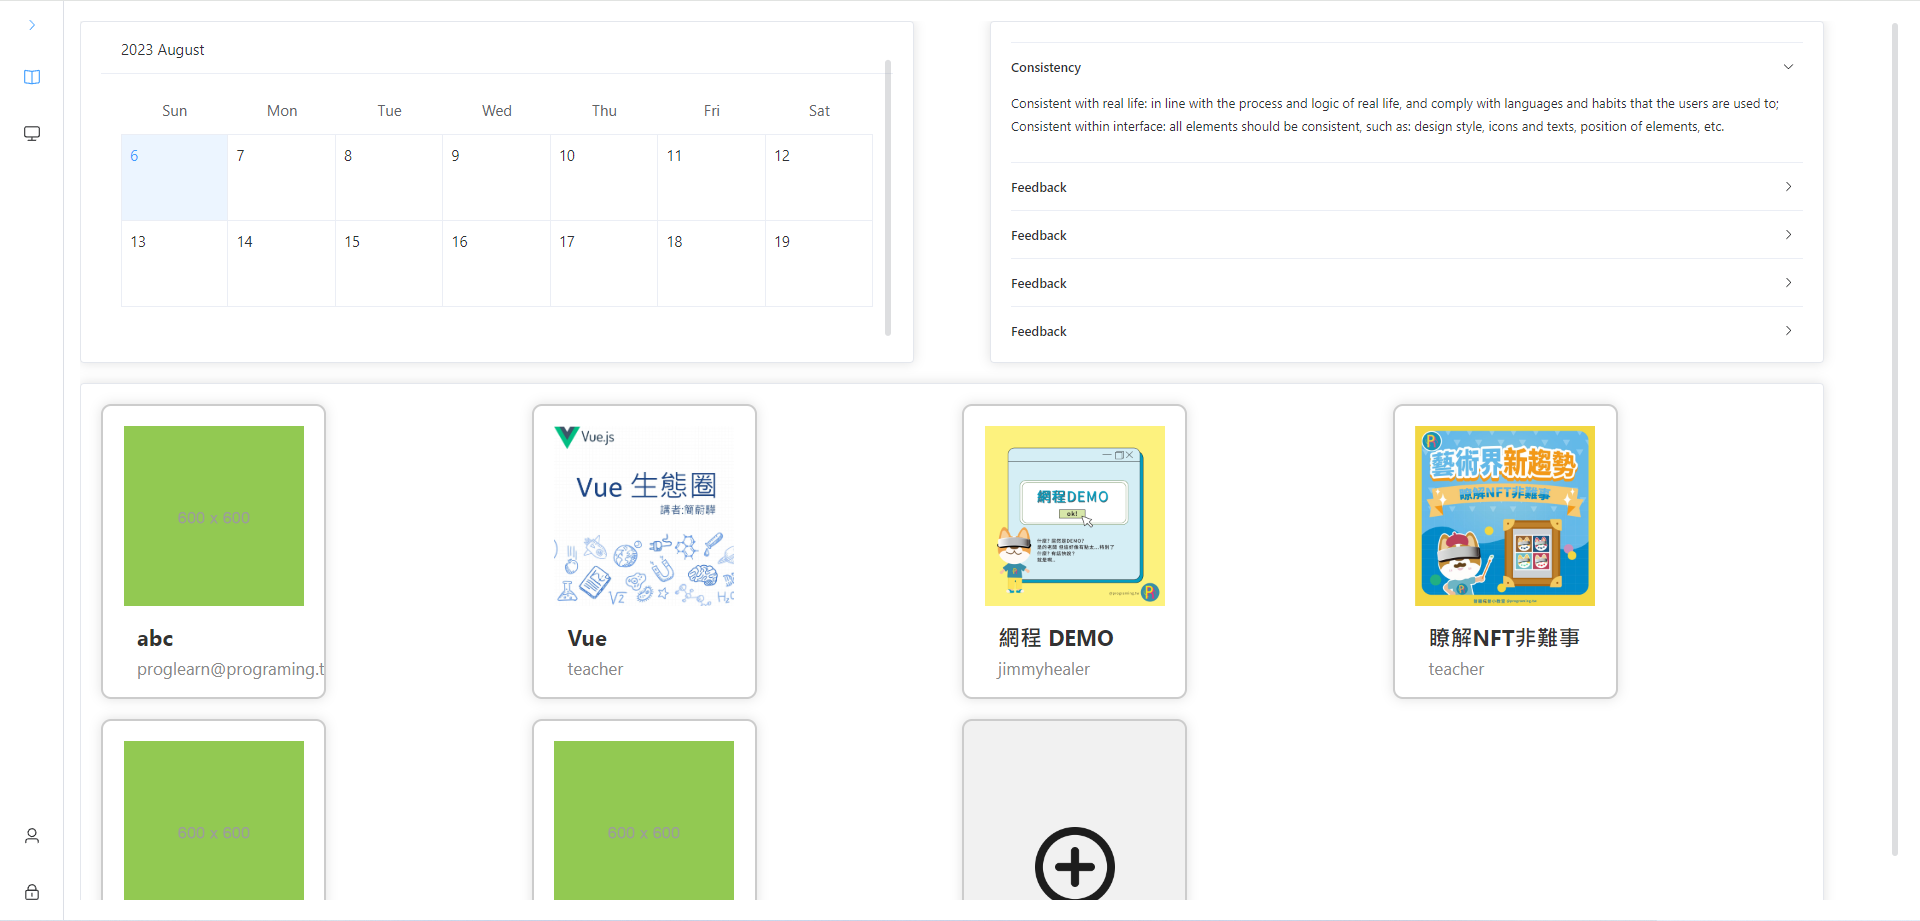
\includegraphics[width=0.75\textwidth]{images/course.png}
    %   }
    \caption{課程清單}
  \end{subfigure}
  \caption{課程相關頁面}
  \label{fig:course}
\end{figure}

\begin{figure}[H]
  \begin{subfigure}{0.5\linewidth}
    \centering
    %   \href{https://raw.githubusercontent.com/programingtw/proglearn-plan/main/img/list.png}{ 
    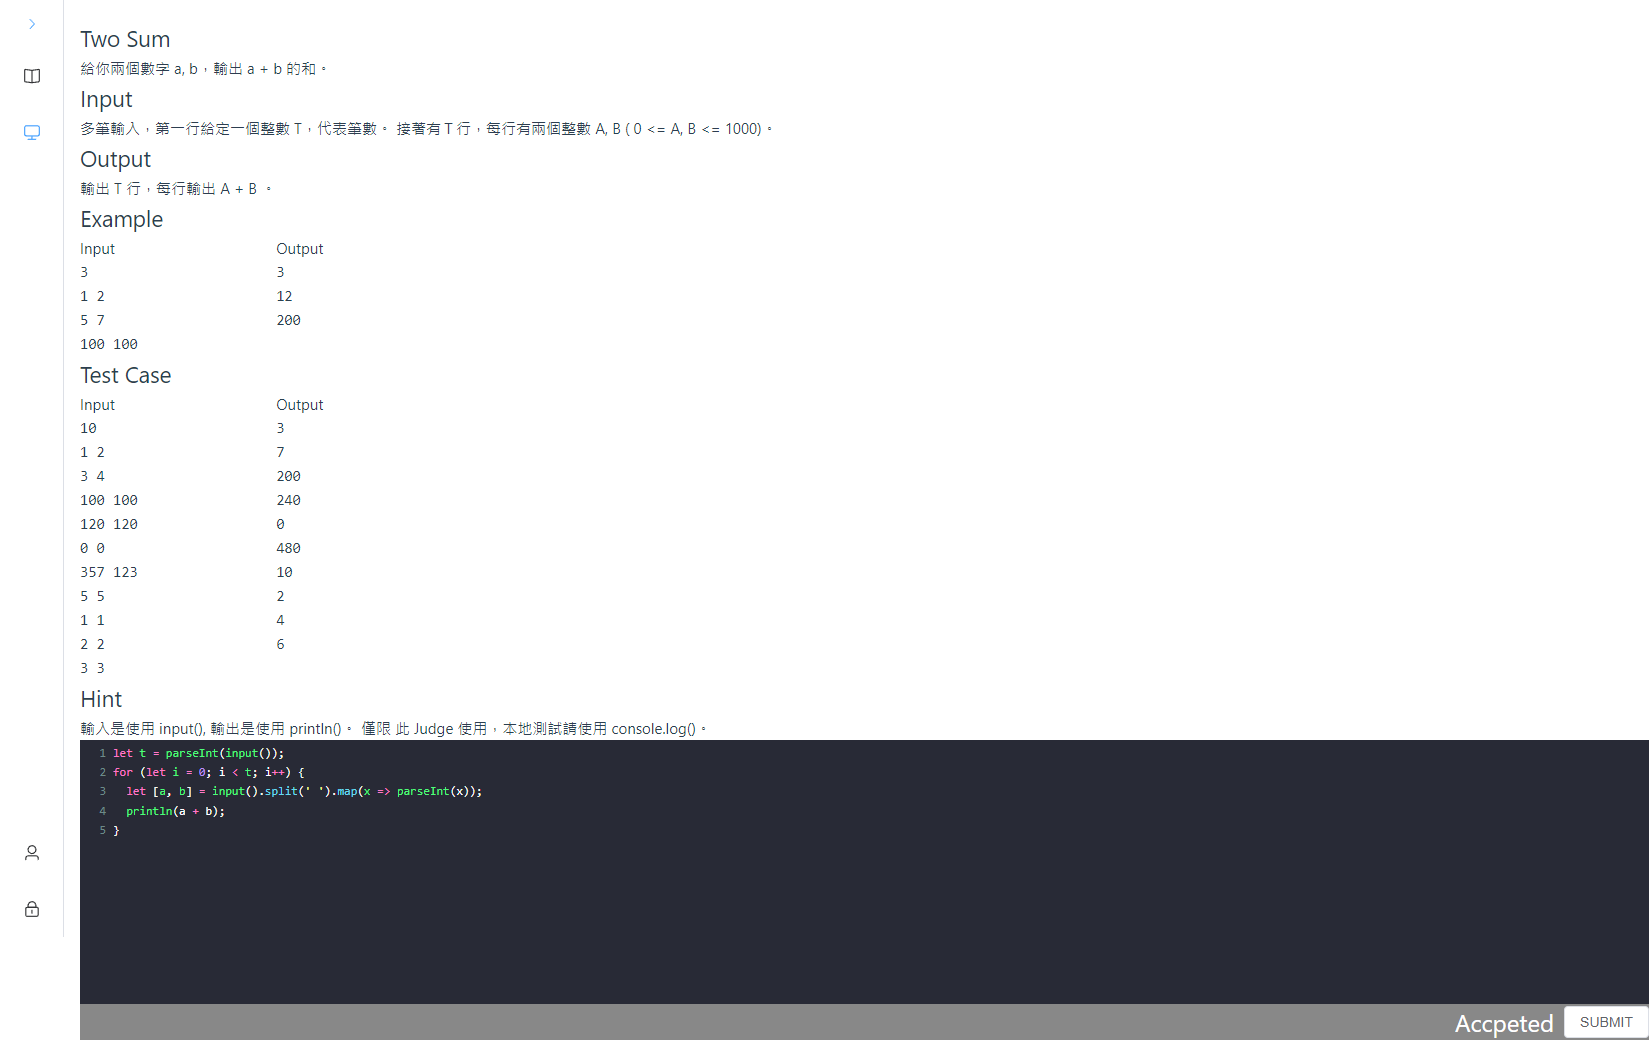
\includegraphics[width=0.75\textwidth]{images/homework.png}
    %   }
    \caption{作業作答}
  \end{subfigure}
  \begin{subfigure}{0.5\linewidth}
    \centering
    %   \href{https://raw.githubusercontent.com/programingtw/proglearn-plan/main/img/course.png}{ 
    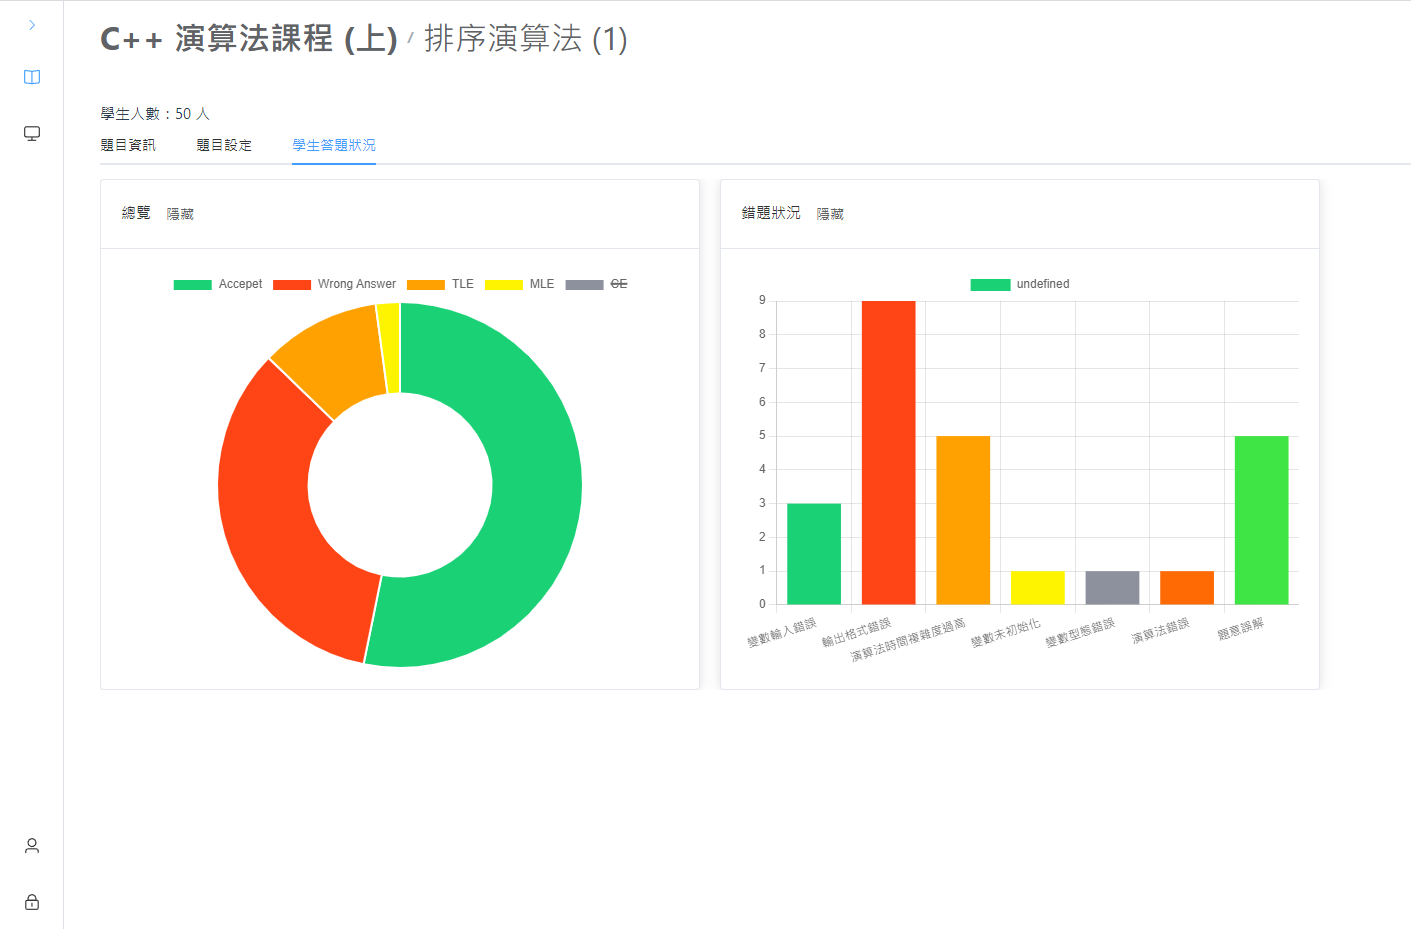
\includegraphics[width=0.75\textwidth]{images/feedback.png}
    %   }
    \caption{作業反饋}
  \end{subfigure}
  \caption{作業相關頁面}
  \label{fig:homework}
\end{figure}

\newpage
\subsection{營運模式}

\begin{figure}[H]
  \centering
  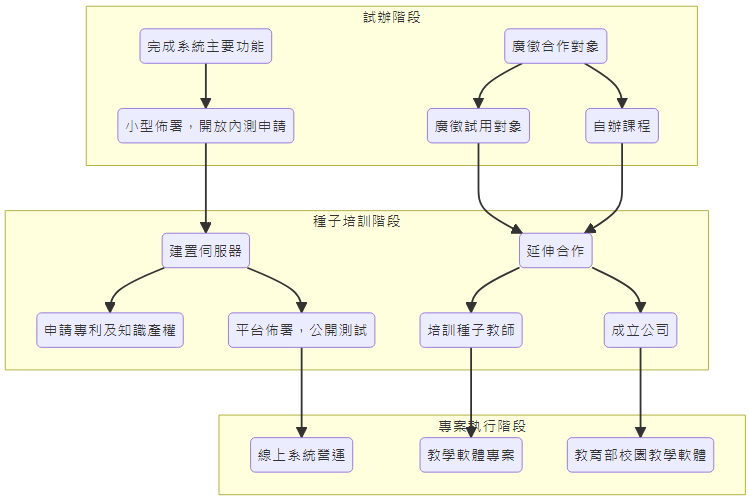
\includegraphics[width=0.8\textwidth]{images/Ops-flow.png}
  \caption{營運模式流程}
\end{figure}

普羅程式將以試辦、種子培訓、專案執行三個階段的營運模式逐步建立起完善的系統服務與客戶群。

在各個階段中,我們將從小範圍逐漸擴大服務與測試的範圍,以確保系統的穩定性以及減少系統營運的成本。同時,蒐集每一階段受試者的反應、使用者的族群,進一步符合市場的需求。
\subsubsection{試辦階段(2024Q2 - 2024Q4)}

試辦階段的主要目的是建立起與目標群眾的信任關係。我們將聚焦於團隊所在地附近的師生,如海洋大學、二信中學,以及曾合作的夥伴學校,如台中市立東山高中與丹鳳高中等廣徵合作的對象,通過免費申請的試用活動,在測試中獲得用戶的反饋。同時,我們也能藉由收集申請人的資料,進一步確認潛在的目標族群。

此外,開發人員將自辦免費的短期教學活動。透過與合作的學校借用場地、設備以及課程的推廣,進行教學活動,以建立與學校的初步合作關係。

\begin{table}[H]
  \centering
  \caption{關鍵活動:廣徵試用對象}
  \begin{tabular}{|l|l|}
      \hline
      \multicolumn{2}{|c|}{\textbf{關鍵活動}} \\ \hline
      活動 & 廣徵試用對象(內測) \\ \hline
      先決條件 & 完成系統的主要功能,並達成小型佈署。 \\ \hline
      參與方式 & 聯繫官方email或line,並填寫使用目的與問卷,普羅程式將由專員進行評估。 \\ \hline
      \multirow{4}{*}{參與條件} & 1. 用於教學目的,需提供課程資訊。 \\
      & 2. 用於公開課程中,需註明普羅程式的資訊。 \\ 
      & 3. 用於公開課程中,需配合普羅程式的使用者調查。 \\ 
      & 4. 用於公開課程中,需提供課程的紀錄與活動照片,並配合普羅程式的宣傳。 \\ \hline
      參與對象 & 海洋大學所有師生(不限年級與科系)。 \\ \hline
      使用方式 & 不限(可用於必選修課程、補強課程、家教教學、讀書會等目的)。 \\ \hline
      執行時間 & 視試用的需求而定,分為週、月、學期等。 \\ \hline
      \multirow{4}{*}{預期效益} & 1. 蒐集使用者的反饋,以改進系統的功能。 \\ 
      & 2. 蒐集使用者的資料,以確認目標族群。 \\ 
      & 3. 建立與使用者的第一層信任關係。 \\
      & 4. 推廣本系統的服務與普羅程式的知名度。 \\ \hline
  \end{tabular}
\end{table}

\begin{table}[H]
  \centering
  \caption{關鍵活動:自辦課程}
  \begin{tabular}{|l|l|}
      \hline
      \multicolumn{2}{|c|}{\textbf{關鍵活動}} \\ \hline
      活動 & 自辦課程 \\ \hline
      先決條件 & 完成系統的主要功能,並達成小型佈署。 \\ \hline
      參與方式 & 由團隊與合作夥伴邀請。 \\ \hline
      \multirow{2}{*}{參與條件} & 1. 普羅程式可以蒐集並運用課程的紀錄與活動照片。 \\
      & 2. 允許使用普羅程式的名義進行課程教學。 \\
      & 3. 需配合普羅程式的使用者調查。 \\ \hline
      參與對象 & 學生。 \\ \hline
      使用方式 & 程式社團、營隊課程。 \\ \hline 
      合作夥伴 & 教學單位(提供教學場所、學生)。 \\ \hline
      執行時間 & 短期(以週為單位)。 \\ \hline 
      過去的合作對象 & 東山高中、海洋大學、丹鳳高中及其高中程式社團等。 \\ \hline
      \multirow{4}{*}{預期效益} & 1. 蒐集使用者的反饋,以改進系統的功能。 \\
      & 2. 蒐集使用者的資料,以確認目標族群。 \\
      & 3. 透過與合作夥伴的合作,建立與學校的合作關係。 \\
      & 4. 推廣本系統的服務與普羅程式的知名度。 \\ \hline
  \end{tabular}
\end{table}

\subsubsection{種子培訓階段(2025Q1 - 2025Q3)}

種子培訓階段的主要目的是,延伸與前一階段的使用者及夥伴的合作,並培育有意願參與的國高中教師,讓其成為我們合作的種子教師,將系統應用於一般的學校課程中,進一步擴大測試與服務的範圍。

並且在該階段,將設立有限公司、商標註冊、提出發明專利申請,以確保系統的知識產權及營運的穩定性,在下一階段的專案執行中,將有助於與學校、教育部建立起B2B的商業關係。

\begin{table}[H]
  \centering
  \caption{種子教師培訓}
  \begin{tabular}{|l|l|}
      \hline
      \multicolumn{2}{|c|}{\textbf{關鍵活動}} \\ \hline
      活動 & 培訓種子教師 \\ \hline
      先決條件 & 完成線上平台佈署,並開放公開測試邀請。 \\ \hline
      參與方式 & 由團隊自行邀請或是自行聯繫官方申請。 \\ \hline
      \multirow{4}{*}{參與條件}       
      & 1. 種子教師需擔任示範課程的教師,將系統應用於自己的實際課程中。\\
      & 2. 於示範課程中,需註明普羅程式的資訊。 \\ 
      & 3. 於示範課程中,需配合普羅程式的使用者調查。 \\ 
      & 4. 於示範課程中,需提供課程的紀錄與活動照片,並配合普羅程式的宣傳。 \\ \hline
      參與對象 & 學校程式課程的教師(包含社團老師、校隊教練)。 \\ \hline
      使用方式 & 將本系統用於國高中課程、大學、社團、校隊等與學校程式教學相關之課程。 \\ \hline 
      合作夥伴 & 教師。 \\ \hline 
      執行時間 & 中期(以學期為單位)。 \\ \hline
      預期合作對象 & 東山高中、丹鳳高中、海大資工、海洋大學。 \\ \hline
      \multirow{4}{*}{預期效益}    
      & 1. 蒐集使用者的反饋,以改進系統的功能。 \\
      & 2. 蒐集使用者的資料,以確認目標族群。 \\
      & 3. 透過與學校單位的合作,加深與學校的信任關係,有助於下一階段的商業合作。 \\
      & 4. 本系統能進入一般的學校課程中,有助於將本系統推廣至更多的學校與合作對象。 \\ \hline
  \end{tabular}
\end{table}

\begin{table}[H]
  \centering
  \caption{公司成立及知識產權申請流程}
  \begin{tabular}{|l|l|}
      \hline
      \multicolumn{2}{|c|}{\textbf{關鍵活動}} \\ \hline
      活動 & 公司成立及知識產權申請 \\ \hline
      參與方式 & 聯繫業師、律師或專利代理人,並進行相應申請程序。 \\ \hline
      \multirow{3}{*}{參與條件}
      & 1. 租借辦公室,設立公司。 \\
      & 2. 完成商標註冊申請,確保公司品牌的合法保護。 \\
      & 3. 完成各技術的使用流程,提出發明專利申請。 \\ \hline
      參與對象 & 公司創辦人、股東、法律代表。 \\ \hline
      使用方式 & 將商標註冊證書及專利申請文件運用於公司商業活動中。 \\ \hline
      合作夥伴 & 相關業師與專利代理機構。 \\ \hline
      執行時間 & 長期(視申請程序及審批時間而定)。 \\ \hline
      \multirow{4}{*}{預期效益}
      & 1. 公司品牌合法保護,避免他人侵權行為。 \\
      & 2. 技術及產品創新保護,提升公司競爭力。 \\
      & 3. 有助於公司的商業合作,提升公司的價值。 \\ 
      & 4. 能夠參與教育部校園數位內容與教學軟體的產品徵求活動,與教育部建立合作關係。 \\ \hline
  \end{tabular}
\end{table}

\subsubsection{專案執行階段(2025Q4 - 2026Q3)}

專案執行階段的主要目的是,在已建立合作關係的學校與教師的基礎上,與他們進行軟體專案的洽談,並以當前的使用案例為參考,尋找新的潛在投資人和合作夥伴。

在該階段,要實現與學校、教師間的交易關係,達成B2B與B2C的商業模式,並進行收費與營利。此外,在成立有限公司及商標註冊後,能夠進一步參與教育部校園數位內容與教學軟體的產品徵求活動,並與教育部建立起長期的合作關係。

\begin{table}[H]
  \centering
  \caption{建立教學軟體專案}
  \begin{tabular}{|l|l|}
      \hline
      \multicolumn{2}{|c|}{\textbf{關鍵活動}} \\ \hline
      活動 & 尋找教學單位,建立教學軟體專案 \\ \hline
      參與方式 & 通過直接聯繫學校、教育機構或教育相關的企業,提出合作提案並商討合作細節 \\ \hline
      \multirow{4}{*}{參與條件} 
      & 1. 與教學單位協商並簽署合同,明確界定雙方的權利和義務 \\ 
      & 2. 教學單位需在課程中,註明是使用普羅程式的授權軟體 \\ 
      & 3. 教學單位需配合普羅程式的使用者調查 \\ 
      & 4. 教學單位需提供課程的紀錄與活動照片,並配合普羅程式的宣傳 \\ \hline
      參與對象 & 學校、補習班、教育培訓機構等教學單位 \\ \hline
      \multirow{3}{*}{使用方式} 
      & 1. 普羅程式授權本系統,並搭配教學單位的課程使用 \\
      & 2. 教學單位可以自行設計課程,並使用本系統的功能 \\
      & 3. 依據合同的內容,普羅程式將提供技術支持,或是提供客製化產品的服務。\\ \hline
      合作夥伴 & 教學單位將成為普羅程式的合作夥伴,共同推動教學軟體專案  \\ \hline
      執行時間 & 長期合作,以年為單位,持續提供技術支持和服務  \\ \hline
      使用場所 & 學校校園內或是教學機構的教室和設施 \\ \hline
      \multirow{3}{*}{預期效益}
      & 1. 透過與教學單位的合作,有助於推廣本系統的服務與普羅程式的知名度 \\
      & 2. 提高市場聲望,有助於與更多的教學單位建立合作關係 \\
      & 3. 實現與學校、教師間的交易關係,達成B2B與B2C的商業模式,取得收益 \\ \hline
  \end{tabular}
\end{table}

% 普羅程式將透過\ref{sec:plan}節(實施方式、時程規劃及預期成效)所提及的自辦、種子輔導、專案執行三個階段的營運模式,逐步建立起完善的系統服務與客戶群。

% % 流程圖:與學校建立合作關係 -> 增加使用案例 -> 與學校建立B2B商業關係
% \begin{figure}[h]
%   \centering
%   \begin{tikzpicture}[node distance=4cm]
  
%       % 第一排
%       \node (start) [startstop] {自辦階段};
%       \node (pro1) [process, right of=start, xshift=2cm] {種子輔導階段};
%       \node (stop) [process, right of=pro1, xshift=2cm] {專案執行階段};
  
%       % 第二排
%       \node (start2) [startstop, below of=start, yshift=2cm] {與學校建立合作關係};
%       \node (pro12) [process, right of=start2, xshift=2cm] {增加使用案例};
%       \node (stop2) [process, right of=pro12, xshift=2cm] {與學校、教師建立起交易關係};
  
%       % 箭頭
%       \draw [arrow] (start) -- (pro1);
%       \draw [arrow] (pro1) -- (stop);
  
%       \draw [arrow] (start2) -- (pro12);
%       \draw [arrow] (pro12) -- (stop2);
  
%   \end{tikzpicture}
%   \caption{營運模式的流程圖}
% \end{figure}

% \begin{enumerate}
%   \setlength{\parindent}{2em}
%   \item 自辦階段:由開發人員自辦教學活動,以建立與學校的初步合作關係。
%   \item 種子輔導階段:培育有意願參與的國高中教師,讓他們成為我們合作的種子教師,並建立更多Proglearn程式教學系統的使用案例。
%   \item 專案執行階段:在已建立合作關係的學校與教師的基礎上,與他們進行軟體專案的洽談,並以當前的使用案例為參考,尋找新的潛在投資人和合作夥伴。
% \end{enumerate}

% 自辦階段與種子輔導階段的主要目的,是建立起與目標群眾(國高中教師及其學校)的信任與合作關係,以進入教育市場。接著,在專案執行階段,建立起與學校、教師間的交易關係,分別以B2B\footnote{B2B:Business to Business,指企業對企業的商業模式。}與B2C\footnote{B2C:Business to Consumer,指企業對消費者的商業模式。}的商業模式進行收費(詳見\ref{sec:revenue}營收模式)。

\subsection{營收模式} % 收益流
% \label{sec:revenue}
% 針對不同種類的用戶實行不同的收費模式,分為B2B(學校端)與B2C(教師端)兩種收費模式:

% \begin{enumerate}
%   \setlength{\parindent}{2em}
%   \item B2B(學校端)
%   \par 針對學校、補教業者等機構提供專案設計與程式教學系統建置的服務。協助機構架設教學系統於自家伺服器上,並提供技術支援。收費模式為一次性專案設計費用與年度授權費用,其費用依據機構規模與教師使用人數而定。
%   \item B2C(教師端)
%   \par 針對個體教師提供教學系統的服務。在我們建置的線上教學系統上,提供教師月訂閱制的付費帳號,並提供技術支援。收費模式為月訂閱制費用,其費用依據學生使用人數而定。
% \end{enumerate}

